\chapter{Conception et développement de l'application SmartCar Ops}

\chapintro
Ce chapitre présente \app, l'application web de supervision qui réunit les deux autres briques du projet : elle
reçoit les images du prototype et de la caméra embarquée, exécute les modèles de détection, enregistre et priorise
les obstacles, et les met à la disposition de l'opérateur. Nous décrivons d'abord ses objectifs, ses choix
technologiques et son architecture, puis la gestion des données, avant de présenter chacune des huit pages. Nous
terminons par une synthèse des interactions entre les modules.

% =================================================================================================
\section{Présentation générale de l'application}

\subsection{Objectifs et fonctionnalités principales}
\app{} a pour objectif de donner à un opérateur une vue complète et à jour de la situation : où sont les véhicules,
ce qu'ils voient, quels obstacles ont été détectés, lesquels sont les plus dangereux et quel itinéraire les évite.
Ses fonctionnalités principales sont :
\begin{itemize}
  \item la supervision en temps réel de la flotte du monde réel et de la voiture du prototype ;
  \item l'affichage des flux vidéo avec les détections des modèles d'IA superposées ;
  \item l'enregistrement, la fusion, l'évaluation de la gravité et la priorisation des obstacles ;
  \item la planification d'itinéraires qui pondère la distance et le risque ;
  \item des statistiques, la présentation des performances des modèles et la surveillance des équipements ;
  \item le basculement instantané entre les environnements \emph{Monde réel} et \emph{Prototype}.
\end{itemize}

\subsection{Choix de Dash et de Plotly}
L'application est développée en Python avec \textbf{Dash}~\cite{dash}, un framework de Plotly qui permet de construire
des applications web analytiques sans écrire de JavaScript. L'interface est décrite par des composants Python
(convertis en composants React dans le navigateur) et son comportement par des \emph{callbacks} : des fonctions
Python déclenchées lorsqu'une entrée change (clic, sélection, minuterie) et qui mettent à jour des sorties.

Ce choix présente plusieurs avantages pour notre projet :
\begin{itemize}
  \item \textbf{un seul langage} pour l'IA, le traitement d'images (OpenCV~\cite{opencv}, ONNX
        Runtime~\cite{onnxruntime}) et l'interface ;
  \item des \textbf{graphiques interactifs} de qualité grâce à Plotly~\cite{plotly} : cartes routières (MapLibre),
        histogrammes, chronologies, cartes de chaleur ;
  \item le \textbf{multi-pages} intégré (\texttt{use\_pages}) et la bibliothèque \textit{Dash Bootstrap Components}
        pour la mise en page ;
  \item un serveur \textbf{Flask} sous-jacent, que nous utilisons aussi pour relayer le flux vidéo.
\end{itemize}

\subsection{Architecture logicielle de l'application}
L'application est organisée en quatre couches (figure~\ref{fig:archi-logicielle}) :
\begin{itemize}
  \item la couche \textbf{présentation} : \texttt{app.py} construit la structure commune (barre latérale, barre
        supérieure, commutateur d'environnement, minuteries), les modules \texttt{pages/} définissent les huit pages
        et leurs callbacks, et \texttt{components/} regroupe le thème, les composants d'interface et les fonctions
        de création de figures ;
  \item la couche \textbf{métier} (\texttt{core/}) : télémétrie en mémoire (\texttt{hub}), obstacles et gravité,
        graphe routier et planification, trajets, journal d'événements, réglages et accès à la base de données ;
  \item la couche \textbf{services} (\texttt{sources/}) : fils d'exécution d'arrière-plan qui lisent la caméra
        ESP32-CAM et les vidéos, exécutent les détecteurs et font tourner les simulateurs ;
  \item la couche \textbf{données} : base SQLite, instantanés et réglages dans un volume Docker, modèles ONNX et
        leurs profils, graphe routier et plan de la piste.
\end{itemize}
L'ensemble s'exécute dans un conteneur Docker~\cite{docker} : la commande \texttt{docker compose up} suffit pour
lancer l'application sur n'importe quelle machine.

\begin{figure}[H]
\centering
\resizebox{\linewidth}{!}{% Architecture logicielle de SmartCar Ops (chapitre 4)
\begin{tikzpicture}[
  m/.style={bloc,font=\footnotesize,minimum height=1.05cm,text width=#1,minimum width=#1},
  m/.default=3.3cm,
  titre/.style={font=\footnotesize\bfseries,text=#1,anchor=south west,inner sep=1pt}]
  % navigateur
  \node[bloc,draw=gris,fill=gris!8,minimum width=15cm,font=\small] (nav) at (7.5,0.6)
       {Navigateur de l'opérateur — interface Dash (React), rafraîchie par \texttt{dcc.Interval} (1 s et 5 s)};
  % présentation
  \node[m=3.3cm,fill=bleufst!8] (appf) at (2.0,-1.5) {\texttt{app.py}\\structure, menu, commutateur};
  \node[m=3.3cm,fill=bleufst!8] (pages) at (5.7,-1.5) {\texttt{pages/}\\8 pages et leurs callbacks};
  \node[m=3.3cm,fill=bleufst!8] (comp) at (9.4,-1.5) {\texttt{components/}\\thème, panneaux, figures};
  \node[m=3.3cm,fill=bleufst!8] (flask) at (13.1,-1.5) {Serveur Flask\\relais vidéo, instantanés};
  % métier
  \node[m=2.6cm,fill=vertfst!12,draw=vertfst!80!black] (hub) at (1.65,-3.6) {\texttt{hub}\\télémétrie en mémoire};
  \node[m=2.6cm,fill=vertfst!12,draw=vertfst!80!black] (obs) at (4.55,-3.6) {\texttt{obstacles}\\\texttt{severity}};
  \node[m=2.6cm,fill=vertfst!12,draw=vertfst!80!black] (plan) at (7.45,-3.6) {\texttt{planner}, \texttt{network}\\(NetworkX)};
  \node[m=2.6cm,fill=vertfst!12,draw=vertfst!80!black] (trips) at (10.35,-3.6) {\texttt{trips}, \texttt{events}\\\texttt{metrics}};
  \node[m=2.6cm,fill=vertfst!12,draw=vertfst!80!black] (set) at (13.25,-3.6) {\texttt{settings}\\\texttt{db} (SQLite)};
  % services
  \node[m=2.6cm,fill=orangefst!12,draw=orangefst] (cam) at (1.65,-5.7) {\texttt{camera}\\découverte, relais};
  \node[m=2.6cm,fill=orangefst!12,draw=orangefst] (perc) at (4.55,-5.7) {\texttt{perception}\\ArUco, mouvement};
  \node[m=2.6cm,fill=orangefst!12,draw=orangefst] (dash) at (7.45,-5.7) {\texttt{dashcam}\\distance, réaction};
  \node[m=2.6cm,fill=orangefst!12,draw=orangefst] (det) at (10.35,-5.7) {\texttt{detector}\\\texttt{onnx\_yolo}};
  \node[m=2.6cm,fill=orangefst!12,draw=orangefst] (sim) at (13.25,-5.7) {\texttt{sim\_real}\\\texttt{sim\_proto}};
  % données
  \node[m=3.3cm,fill=gris!10,draw=gris] (sqlite) at (2.0,-7.8) {Volume \texttt{/data}\\SQLite, instantanés};
  \node[m=3.3cm,fill=gris!10,draw=gris] (models) at (5.7,-7.8) {\texttt{models/}\\ONNX, profils, registre};
  \node[m=3.3cm,fill=gris!10,draw=gris] (res) at (9.4,-7.8) {\texttt{resources/}\\graphe OSM, piste};
  \node[m=3.3cm,fill=gris!10,draw=gris] (vid) at (13.1,-7.8) {\texttt{demo/videos}\\+ flux ESP32-CAM};
  % couches
  \begin{scope}[on background layer]
    \node[zone,fill=bleufst!4,fit=(appf)(flask)] (z1) {};
    \node[zone,fill=vertfst!5,fit=(hub)(set)] (z2) {};
    \node[zone,fill=orangefst!5,fit=(cam)(sim)] (z3) {};
    \node[zone,fill=gris!5,fit=(sqlite)(vid)] (z4) {};
    \node[draw=encre,thick,rounded corners=8pt,inner sep=8pt,fit=(z1)(z4),
          label={[font=\small\bfseries,anchor=north east]south east:Conteneur Docker \texttt{iot-smartcar-dashboard}}] {};
  \end{scope}
  \node[titre=bleufst] at (z1.north west) {Présentation};
  \node[titre=vertfst!60!black] at (z2.north west) {Métier (\texttt{core/})};
  \node[titre=orangefst!80!black] at (z3.north west) {Services d'arrière-plan (\texttt{sources/})};
  \node[titre=gris] at (z4.north west) {Données};
  \draw[fleche,{Stealth[length=2.6mm]}-{Stealth[length=2.6mm]}] (pages.north |- nav.south) -- (pages.north);
  \draw[fleche] (flask.north) -- (flask.north |- nav.south);
\end{tikzpicture}
}
\caption{Architecture logicielle de \app}
\label{fig:archi-logicielle}
\end{figure}

\subsection{Organisation de l'interface et navigation}
L'interface suit une organisation classique de tableau de bord. À gauche, une barre latérale flottante regroupe les
huit pages par thème (figure~\ref{fig:sidebar}) : \textbf{Live} (Tracking, Camera), \textbf{Planning} (Route
planner), \textbf{Safety} (Obstacles), \textbf{Analytics} (Live stats, AI models) et \textbf{System} (Devices \&
logs), la page \textbf{Overview} étant placée en tête. Une horloge et un voyant d'activité figurent en bas de la
barre. En haut, une barre affiche le titre et la description de la page courante, l'état de la source de données et
le commutateur d'environnement.

\begin{figure}[H]
\centering
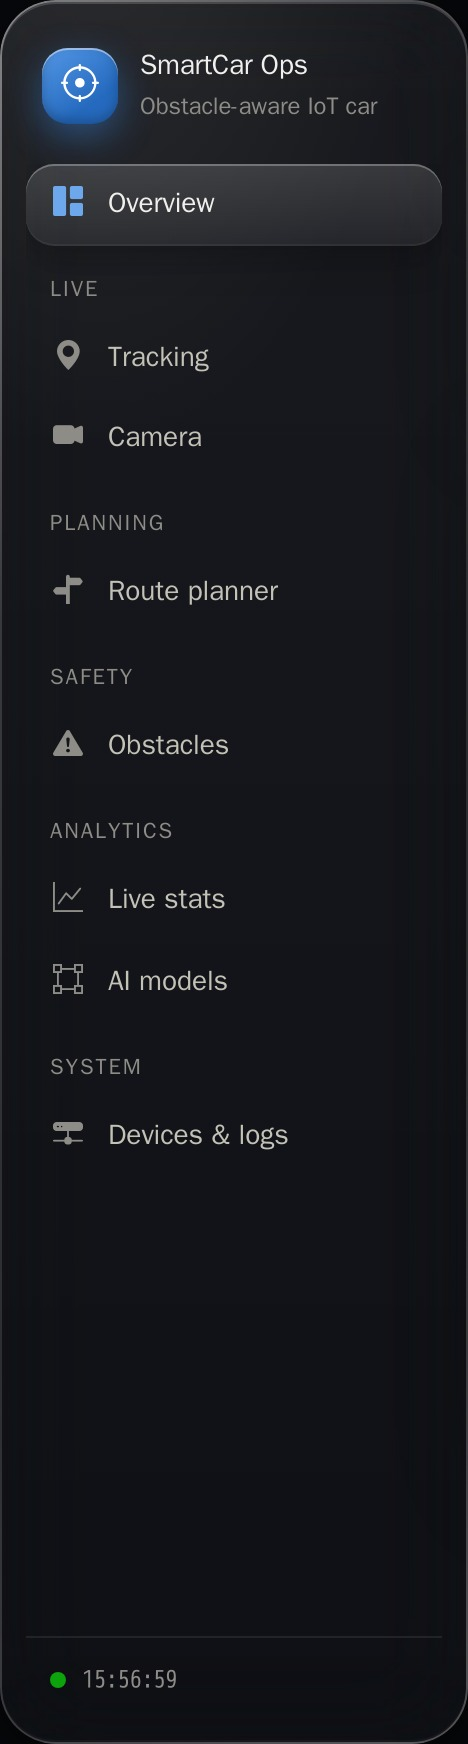
\includegraphics[height=8.6cm]{captures/sidebar.jpg}
\caption{Menu latéral complet de l'application}
\label{fig:sidebar}
\end{figure}

\subsection{Gestion des deux environnements : Real World et Prototype}
Le commutateur de la barre supérieure fait basculer toute l'application entre les deux environnements
(figure~\ref{fig:switch}). Sa valeur est mémorisée dans le navigateur et transmise à chaque callback : chaque page
interroge alors les données de l'environnement choisi et adapte son contenu. Les unités passent des mètres aux
centimètres, la carte routière de Paris laisse place au plan de la piste, et les indicateurs propres à la flotte
(batterie, nombre de véhicules) sont remplacés par ceux du prototype (état de la voiture, progression du parcours,
cadence de la caméra). L'indicateur de source précise l'origine des données : \emph{Simulated data} pour le monde
réel, \emph{Live · ESP32-CAM} lorsque la caméra du prototype est connectée, ou \emph{Demo} lorsqu'elle ne l'est pas.

\begin{figure}[H]
\centering
\begin{subfigure}[b]{\linewidth}\centering
  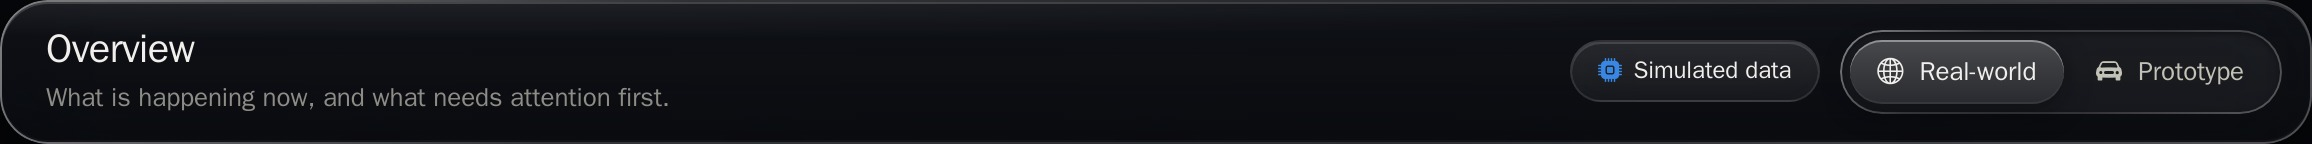
\includegraphics[width=\linewidth]{captures/topbar_real.jpg}
  \caption{Environnement \emph{Real-world}}
\end{subfigure}

\vspace{0.2cm}
\begin{subfigure}[b]{\linewidth}\centering
  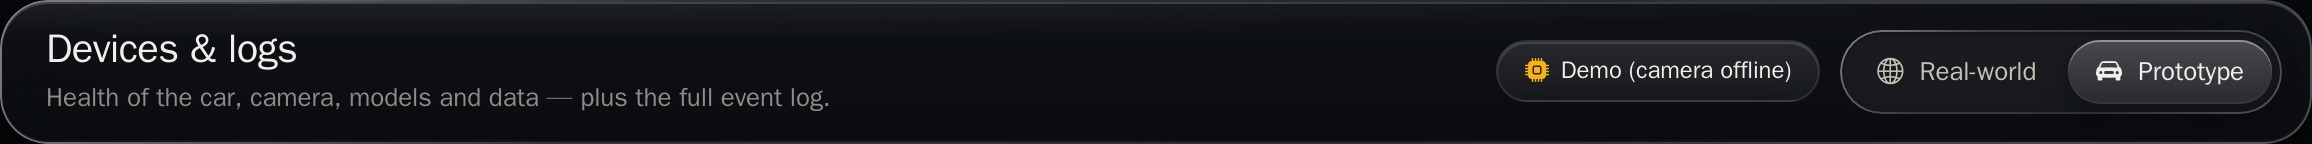
\includegraphics[width=\linewidth]{captures/topbar_proto.jpg}
  \caption{Environnement \emph{Prototype}}
\end{subfigure}

\vspace{0.2cm}
\begin{subfigure}[b]{0.49\linewidth}\centering
  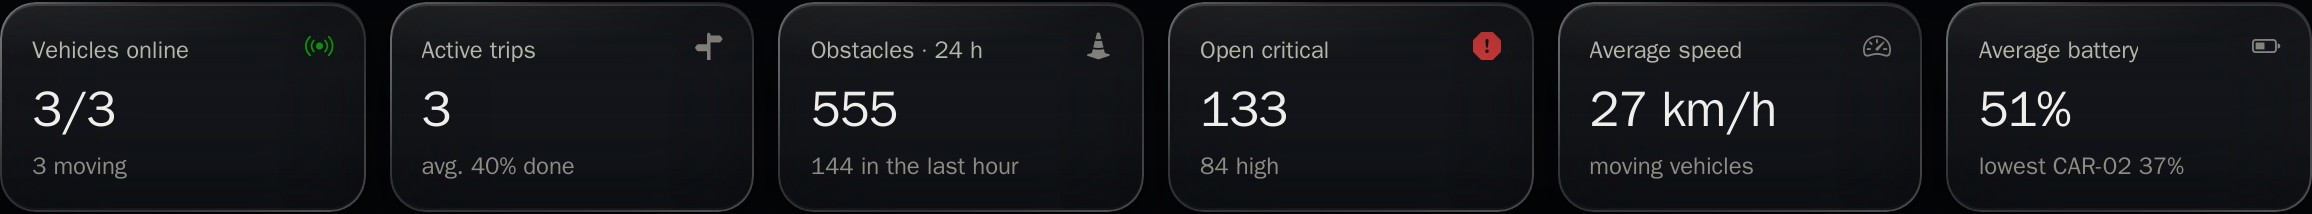
\includegraphics[width=\linewidth]{captures/overview_kpi_real.jpg}
  \caption{Indicateurs de la flotte (monde réel)}
\end{subfigure}\hfill
\begin{subfigure}[b]{0.49\linewidth}\centering
  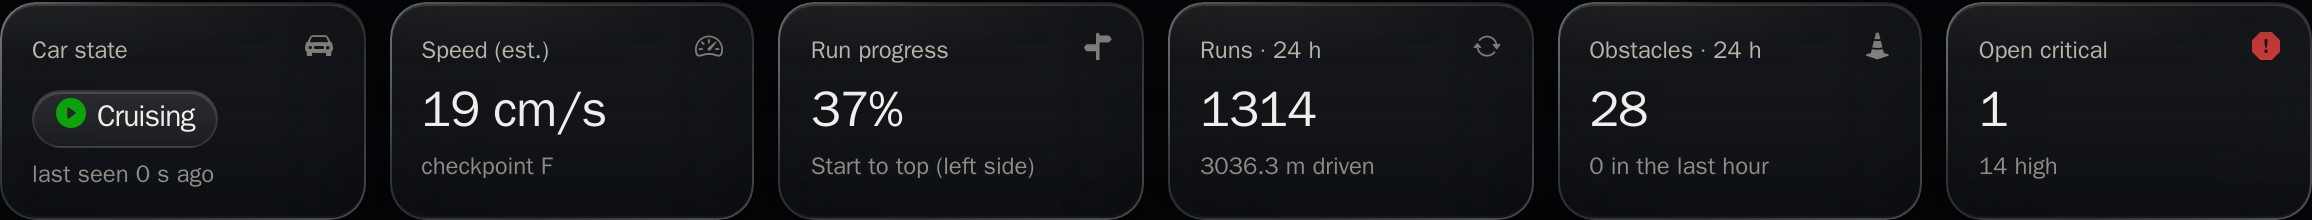
\includegraphics[width=\linewidth]{captures/overview_kpi_proto.jpg}
  \caption{Indicateurs de la voiture (prototype)}
\end{subfigure}
\caption{Changement d'environnement : barre supérieure et indicateurs de la page Overview}
\label{fig:switch}
\end{figure}

% =================================================================================================
\section{Architecture et gestion des données}

\subsection{Architecture générale des échanges de données}
La figure~\ref{fig:flux} décrit la circulation des données. Les \emph{sources} (caméra ESP32-CAM, vidéos de la
caméra embarquée, simulateurs) sont lues par des services qui s'exécutent en arrière-plan, indépendamment des
pages. Les images passent par les détecteurs ; les résultats sont enregistrés dans deux espaces de stockage : un
\textbf{hub en mémoire} pour les données très volatiles (position et état courants des véhicules, dernières
détections) et la \textbf{base SQLite} pour les données à conserver (obstacles, trajets, points de trajectoire,
événements). Les pages lisent ces données à chaque rafraîchissement ; le flux vidéo annoté est servi directement par
le serveur Flask.

\begin{figure}[H]
\centering
\resizebox{\linewidth}{!}{% Flux de données entre les composants (chapitre 4)
\begin{tikzpicture}[
  s/.style={bloc,font=\footnotesize,minimum width=3.0cm,text width=2.8cm,minimum height=1.05cm},
  lb/.style={font=\scriptsize\itshape,text=gris,fill=white,inner sep=1pt},
  col/.style={font=\footnotesize\bfseries,text=gris}]
  % titres de colonnes
  \node[col] at (0,1.15) {Sources}; \node[col] at (4.2,1.15) {Services d'arrière-plan};
  \node[col] at (8.2,1.15) {Modèles}; \node[col] at (12.6,1.15) {Stockage};
  % sources
  \node[s,fill=orangefst!12,draw=orangefst] (esp) at (0,0) {ESP32-CAM\\flux vidéo Wi-Fi};
  \node[s,fill=vertfst!12,draw=vertfst!80!black] (vid) at (0,-1.9) {Vidéos de route\\(dashcam CAR-01)};
  \node[s,fill=gris!8,draw=gris] (sims) at (0,-3.8) {Simulateurs\\(flotte, démo prototype)};
  % services
  \node[s,fill=bleufst!10] (camsvc) at (4.2,0) {Service caméra\\rotation, ArUco, mouvement};
  \node[s,fill=bleufst!10] (dcs) at (4.2,-1.9) {Service dashcam\\distance, voie, réaction};
  % modèles
  \node[s,fill=bleufst!18] (onnx) at (8.2,-0.95) {Détecteurs YOLO26\\(ONNX Runtime)};
  % stockage
  \node[s,fill=gris!10,draw=gris] (hub) at (12.6,0) {Hub en mémoire\\télémétrie, détections};
  \node[s,fill=gris!10,draw=gris] (db) at (12.6,-1.9) {SQLite : obstacles, trajets, événements};
  \node[s,fill=gris!10,draw=gris] (snap) at (12.6,-3.8) {Instantanés JPEG\\(volume \texttt{/data})};
  % consommateurs
  \node[bloc,font=\footnotesize,minimum width=15.6cm,fill=fond] (ui) at (6.3,-5.9)
       {Callbacks Dash (1 s / 5 s) $\rightarrow$ 8 pages \quad | \quad relais MJPEG annoté $\rightarrow$ page Camera
        \quad | \quad planificateur : risque des segments};
  % flux
  \draw[fleche] (esp) -- node[lb,above] {JPEG} (camsvc);
  \draw[fleche] (vid) -- node[lb,above] {images} (dcs);
  \draw[fleche,{Stealth[length=2.4mm]}-{Stealth[length=2.4mm]}] (camsvc.south east) -- node[lb,above,sloped,pos=0.45] {image / boîtes} (onnx.north west);
  \draw[fleche,{Stealth[length=2.4mm]}-{Stealth[length=2.4mm]}] (dcs.north east) -- node[lb,below,sloped,pos=0.45] {image / boîtes} (onnx.south west);
  % bus vers le stockage
  \coordinate (bus) at (10.45,0);
  \draw[very thick,draw=encre] (10.45,0) -- (10.45,-3.8);
  \draw[thick,draw=encre] (camsvc.east) -- node[lb,above,pos=0.55] {position, état, détections} (10.45,0);
  \draw[thick,draw=encre] (dcs.east) -- node[lb,below,pos=0.55] {obstacles, réactions} (10.45,-1.9);
  \draw[thick,draw=encre] (sims.east) -- node[lb,above,pos=0.6] {télémétrie, obstacles simulés} (10.45,-3.8);
  \foreach \n in {hub,db,snap} \draw[fleche] (bus |- \n.west) -- (\n.west);
  % vers l'interface
  \draw[fleche] (hub.east) -- ++(0.35,0) |- ([yshift=0.15cm]ui.east);
  \draw[thick,draw=encre] (db.east) -- ++(0.35,0);
  \draw[fleche] (snap.south) -- (snap.south |- ui.north);
\end{tikzpicture}
}
\caption{Flux des données entre les composants de \app}
\label{fig:flux}
\end{figure}

\subsection{Intégration des modèles YOLO26}
Les modèles sont chargés une seule fois, au démarrage des services, à partir de leurs profils
(chapitre~3) : le service de la caméra embarquée charge les deux modèles routiers, le service de l'ESP32-CAM le
modèle du prototype. L'inférence s'exécute dans un fil dédié qui analyse toujours l'image la plus récente, sans
bloquer ni la lecture vidéo ni l'interface. Les pages n'appellent jamais directement les modèles : elles lisent
leurs résultats dans le hub et la base de données. La page \emph{AI models} affiche les modèles effectivement chargés
et leur temps d'exécution.

\subsection{Acquisition et traitement des données du prototype}
L'Arduino ne disposant d'aucune liaison sans fil, toutes les données du prototype sont extraites de l'image de
l'ESP32-CAM :
\begin{itemize}
  \item \textbf{Découverte de la caméra} : son adresse IP étant dynamique, le service essaie successivement l'adresse
        saisie dans l'application, celle de la configuration, la dernière adresse qui a fonctionné, puis balaye les
        sous-réseaux configurés en testant en parallèle les ports 80 et 81 et la réponse \texttt{/status}.
  \item \textbf{Relais} : la caméra ne servant qu'un client à la fois, le serveur est son unique client et
        redistribue les images à tous les onglets ouverts par la route \texttt{/camera/stream.mjpg}.
  \item \textbf{Redressement} : l'image est tournée selon le montage de la caméra (90° pour notre prototype).
  \item \textbf{Perception} : les marqueurs ArUco~\cite{garrido2014aruco} imprimés aux points de passage A à F
        indiquent à quel point de la piste se trouve la voiture ; entre deux marqueurs, la position est estimée à
        partir de la vitesse mesurée. La différence entre images successives indique si la voiture roule ou est
        arrêtée. Le détecteur fournit les obstacles.
  \item \textbf{Trajets} : le passage au premier marqueur de la trajectoire active ouvre un trajet, le passage au
        dernier le clôture avec la distance parcourue.
\end{itemize}
Lorsque la caméra est hors ligne, un simulateur de démonstration fait rouler une voiture virtuelle sur la piste, afin
que les pages restent utilisables.

\subsection{Gestion des données issues du monde réel}
L'environnement monde réel s'appuie sur le graphe routier du Quartier Latin à Paris, extrait d'OpenStreetMap~\cite{osm}
(309 intersections, 406 tronçons). Un simulateur fait circuler trois véhicules sur ce graphe : il choisit des
trajets, fait avancer les véhicules à des vitesses réalistes, gère leur batterie et produit des rencontres
d'obstacles plus fréquentes sur les tronçons à risque. Le véhicule CAR-01 fait exception : ses obstacles proviennent
uniquement de sa caméra embarquée, alimentée par de vraies vidéos de route (ou un flux réseau, par exemple un
téléphone fixé sur un tableau de bord) et analysée par les modèles. Chaque obstacle statique détecté est placé sur
la carte devant CAR-01, à la distance estimée, et peut le faire ralentir ou s'arrêter.

\subsection{Organisation et stockage des informations}
Les données persistantes sont stockées dans une base \textbf{SQLite}~\cite{sqlite} en mode WAL (journalisation
anticipée, qui permet des lectures pendant les écritures), placée dans un volume Docker. Elle comporte quatre tables :
\begin{itemize}
  \item \texttt{obstacles} : environnement, classe, confiance, proximité, distance, présence sur la trajectoire,
        position, tronçon, score de gravité, niveau, statut (nouveau, acquitté, résolu, faux positif), nombre
        d'observations, dates de première et dernière observation, instantané, source ;
  \item \texttt{trips} et \texttt{trip\_points} : trajets (véhicule, itinéraire, durée, distance, obstacles
        rencontrés) et points de trajectoire horodatés pour la relecture ;
  \item \texttt{events} : journal des événements (niveau, catégorie, message).
\end{itemize}
Les réglages (adresse de la caméra, rotation, trajectoire active, poids de danger) sont conservés dans un petit
fichier JSON, et les instantanés dans un dossier d'images du même volume.

\subsection{Actualisation des données et affichage en temps réel}
Deux minuteries (\texttt{dcc.Interval}) cadencent l'interface : chaque seconde pour les données en direct (positions,
états, détections, indicateurs) et toutes les cinq secondes pour les vues plus lourdes (statistiques, listes). Seuls
les callbacks de la page affichée sont exécutés. La vidéo, elle, n'utilise pas ce mécanisme : la balise image du
navigateur reçoit directement le flux MJPEG relayé, à la cadence de la caméra.

% =================================================================================================
\section{Page Overview : tableau de bord général}

\subsection{Présentation de la vue d'ensemble}
La page \emph{Overview} est la page d'accueil (figure~\ref{fig:overview_real_ecran}). Elle répond en un coup d'œil à
la question « que se passe-t-il maintenant ? » : une rangée d'indicateurs, une carte en direct, une vignette de la
caméra, la liste des obstacles à traiter et les derniers événements.

\capture{overview_real_ecran}{Tableau de bord général (page Overview, environnement monde réel)}

\subsection{Affichage des indicateurs clés}
En environnement monde réel, les indicateurs sont : le nombre d'obstacles critiques ouverts (et d'obstacles de
niveau élevé), le nombre d'obstacles détectés en 24 heures et dans la dernière heure, les véhicules en ligne et en
mouvement, les trajets en cours, la vitesse moyenne et la batterie moyenne de la flotte. En mode prototype, ils
deviennent l'état de la voiture, sa vitesse estimée, la progression du parcours et le nombre de parcours des
dernières 24 heures (figure~\ref{fig:switch}).

\subsection{Synthèse des véhicules et des obstacles}
La carte en direct montre les véhicules, colorés selon leur état (en route, en évitement, arrêté) et les obstacles
ouverts. Le panneau \emph{Needs attention} liste les obstacles ouverts du plus grave au moins grave et le panneau
\emph{Recent events} les derniers événements : arrivée d'un véhicule, obstacle critique, connexion de la caméra…
(figure~\ref{fig:overview-panels}).

\begin{figure}[H]
\centering
\begin{subfigure}[b]{0.49\linewidth}\centering
  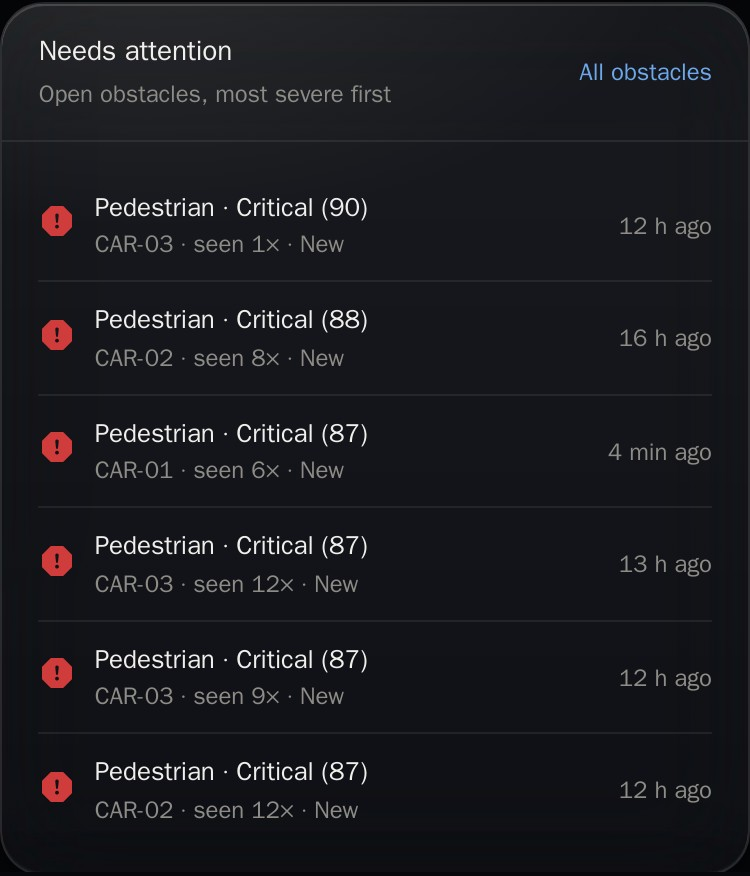
\includegraphics[width=\linewidth]{captures/overview_attention.jpg}
  \caption{Obstacles à traiter}
\end{subfigure}\hfill
\begin{subfigure}[b]{0.49\linewidth}\centering
  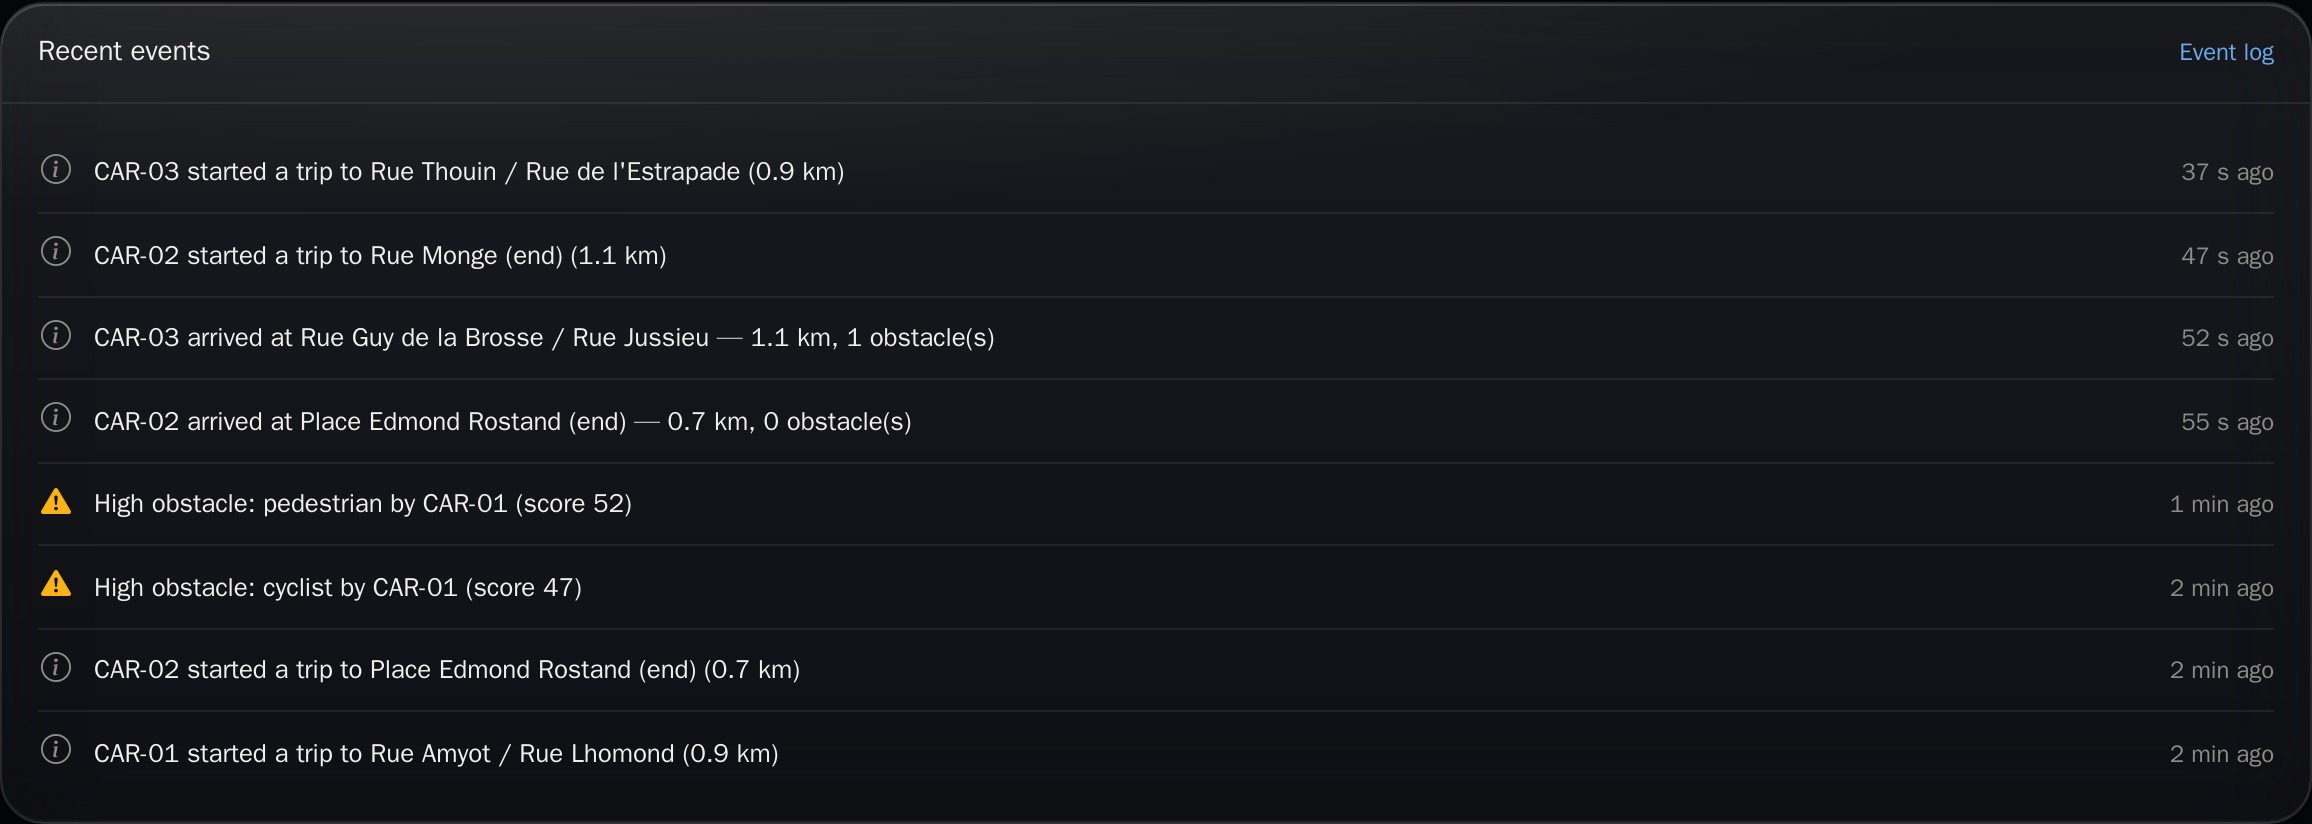
\includegraphics[width=\linewidth]{captures/overview_events.jpg}
  \caption{Événements récents}
\end{subfigure}
\caption{Synthèse des obstacles et des événements de la page Overview}
\label{fig:overview-panels}
\end{figure}

\subsection{Comparaison des environnements Real World et Prototype}
La structure de la page est identique dans les deux environnements, ce qui facilite la prise en main. Seuls le fond
de carte et les indicateurs changent : carte routière et flotte de trois véhicules d'un côté, plan de la piste et
voiture unique de l'autre (figure~\ref{fig:overview-maps}).

\begin{figure}[H]
\centering
\begin{subfigure}[b]{0.49\linewidth}\centering
  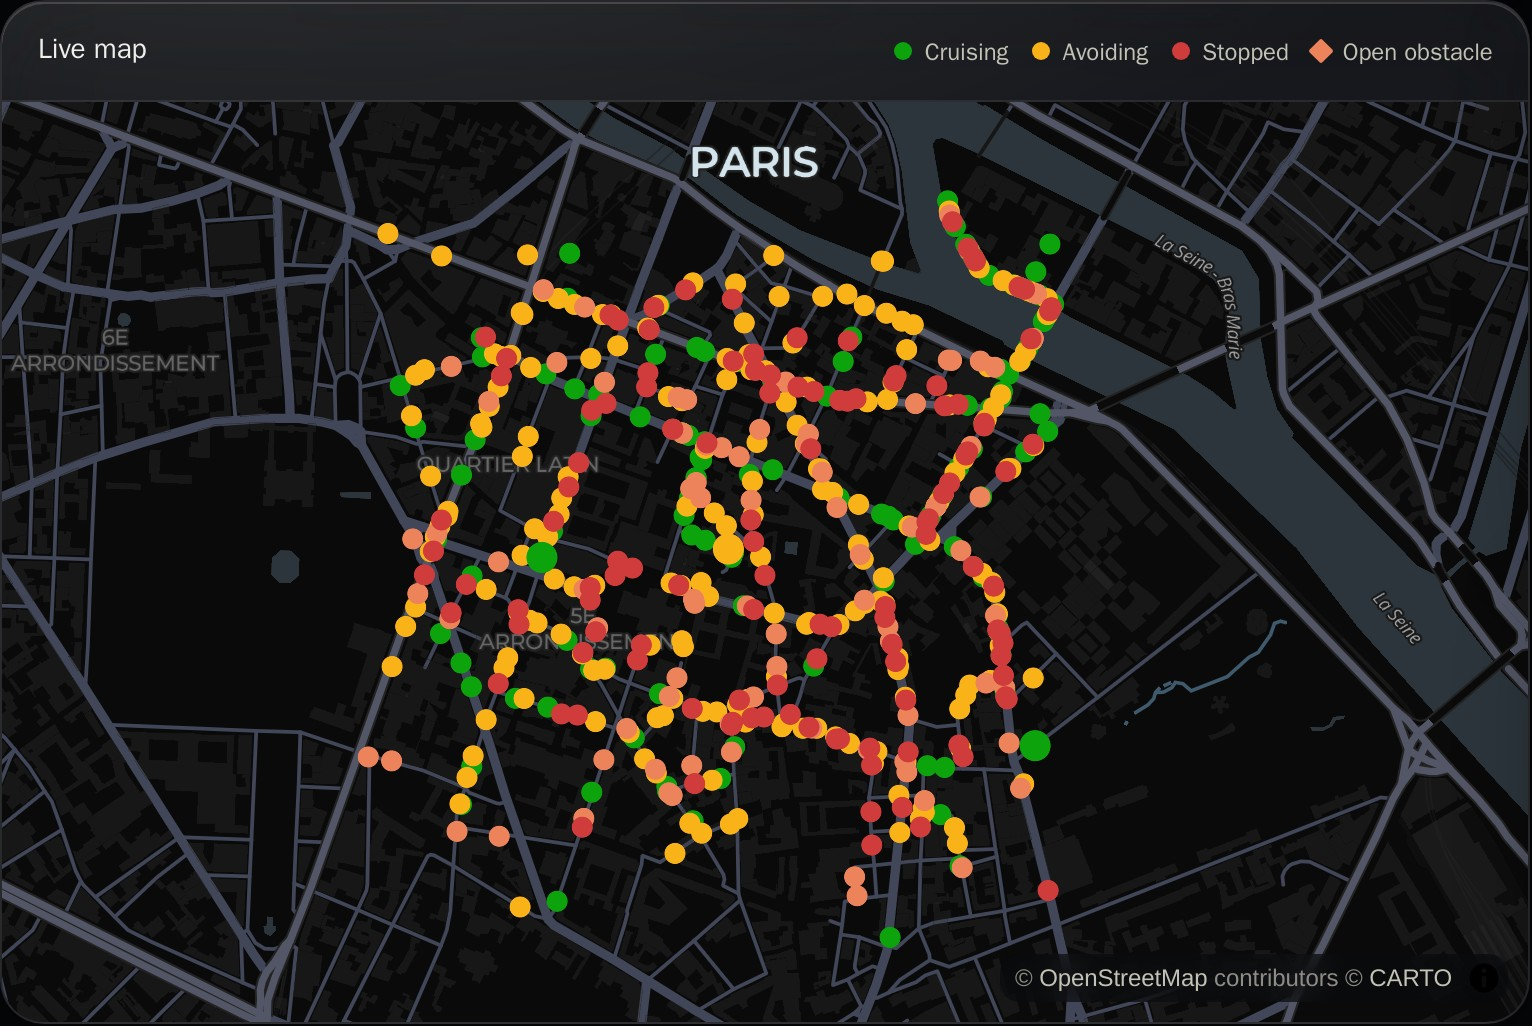
\includegraphics[width=\linewidth]{captures/overview_map_real.jpg}
  \caption{Monde réel : Quartier Latin}
\end{subfigure}\hfill
\begin{subfigure}[b]{0.49\linewidth}\centering
  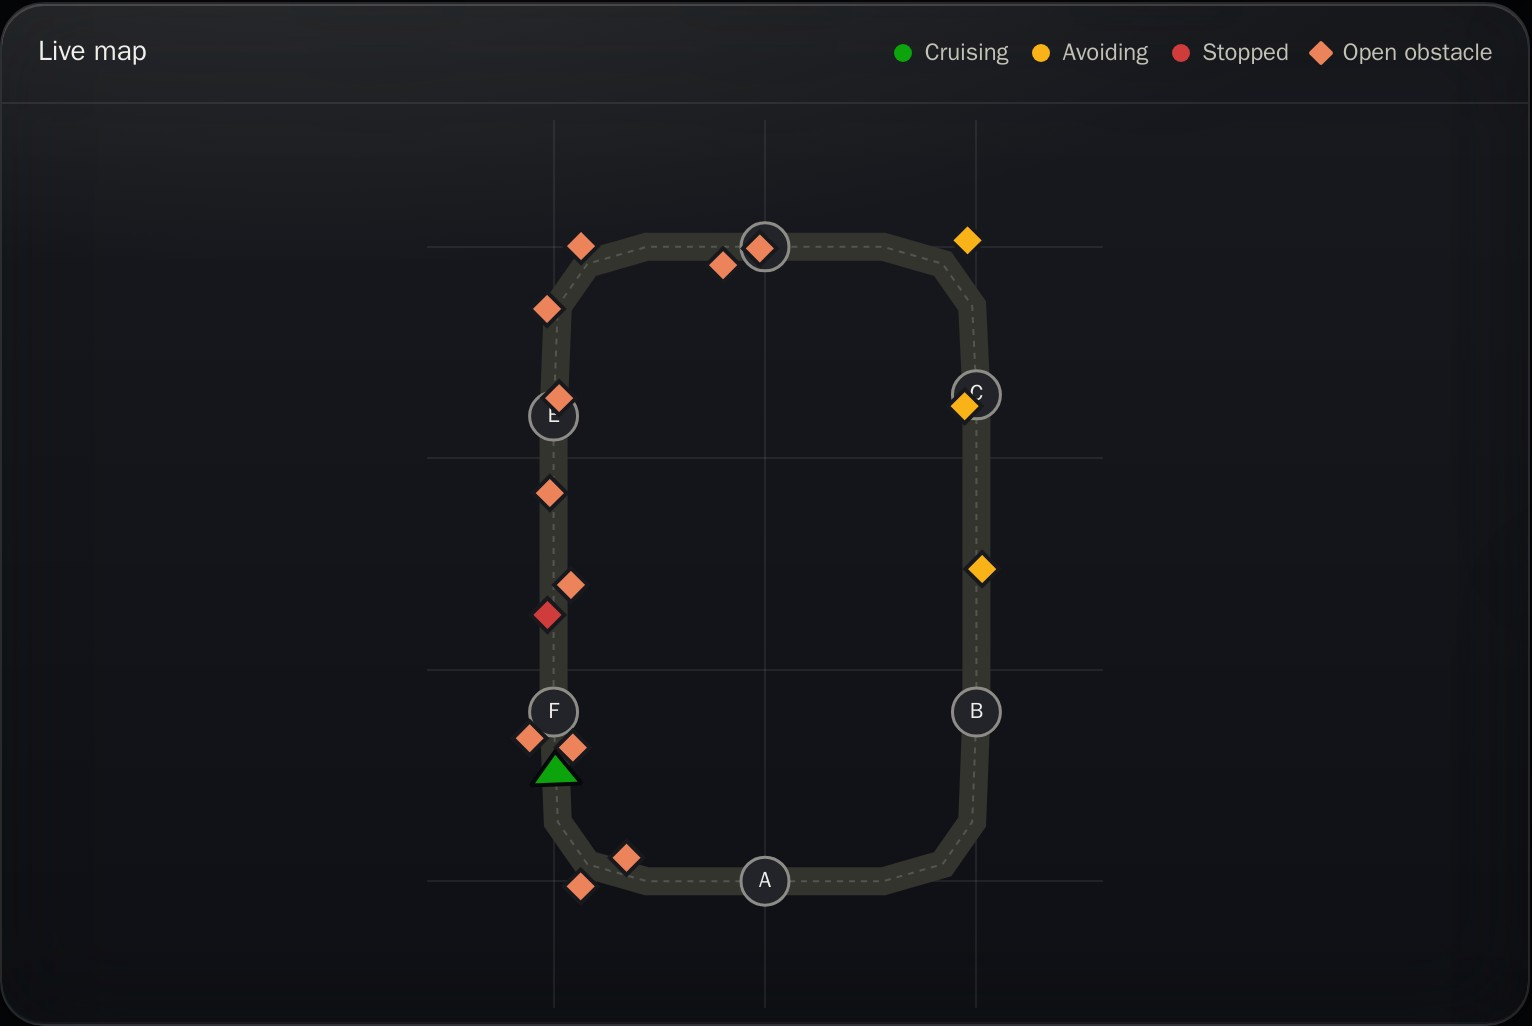
\includegraphics[width=\linewidth]{captures/overview_map_proto.jpg}
  \caption{Prototype : plan de la piste}
\end{subfigure}
\caption{Carte en direct dans les deux environnements}
\label{fig:overview-maps}
\end{figure}

% =================================================================================================
\section{Page Tracking : suivi et localisation des véhicules}

\subsection{Visualisation de la position des véhicules}
La carte de la page \emph{Tracking} affiche la position de chaque véhicule, rafraîchie chaque seconde, avec une
flèche indiquant sa direction (figure~\ref{fig:tracking-map}). Le véhicule sélectionné est mis en évidence. Dans le
prototype, la position est donnée sur le plan de la piste, avec les points de passage A à F.

\begin{figure}[H]
\centering
\begin{subfigure}[b]{0.49\linewidth}\centering
  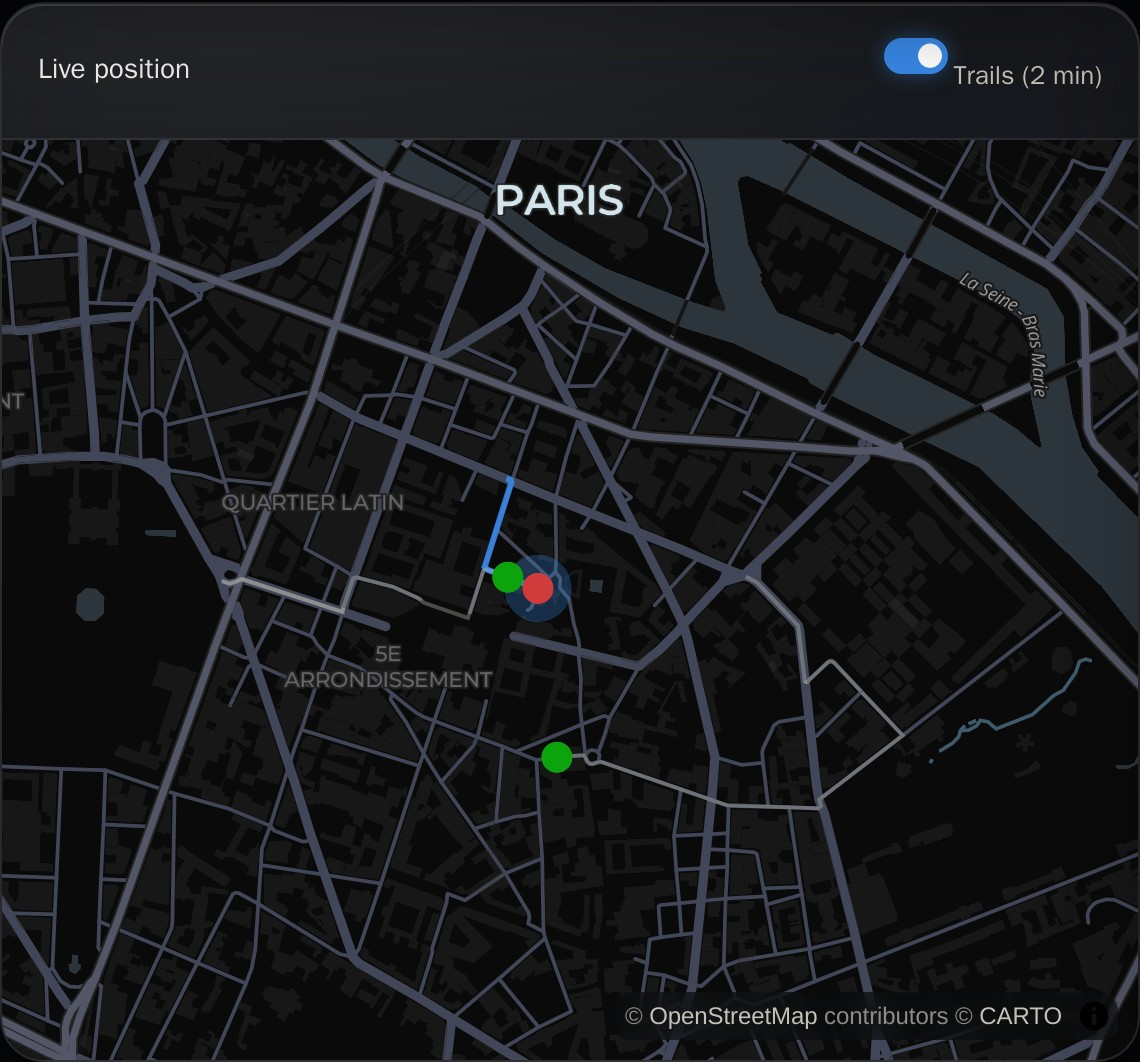
\includegraphics[width=\linewidth]{captures/tracking_map_real.jpg}
  \caption{Monde réel}
\end{subfigure}\hfill
\begin{subfigure}[b]{0.49\linewidth}\centering
  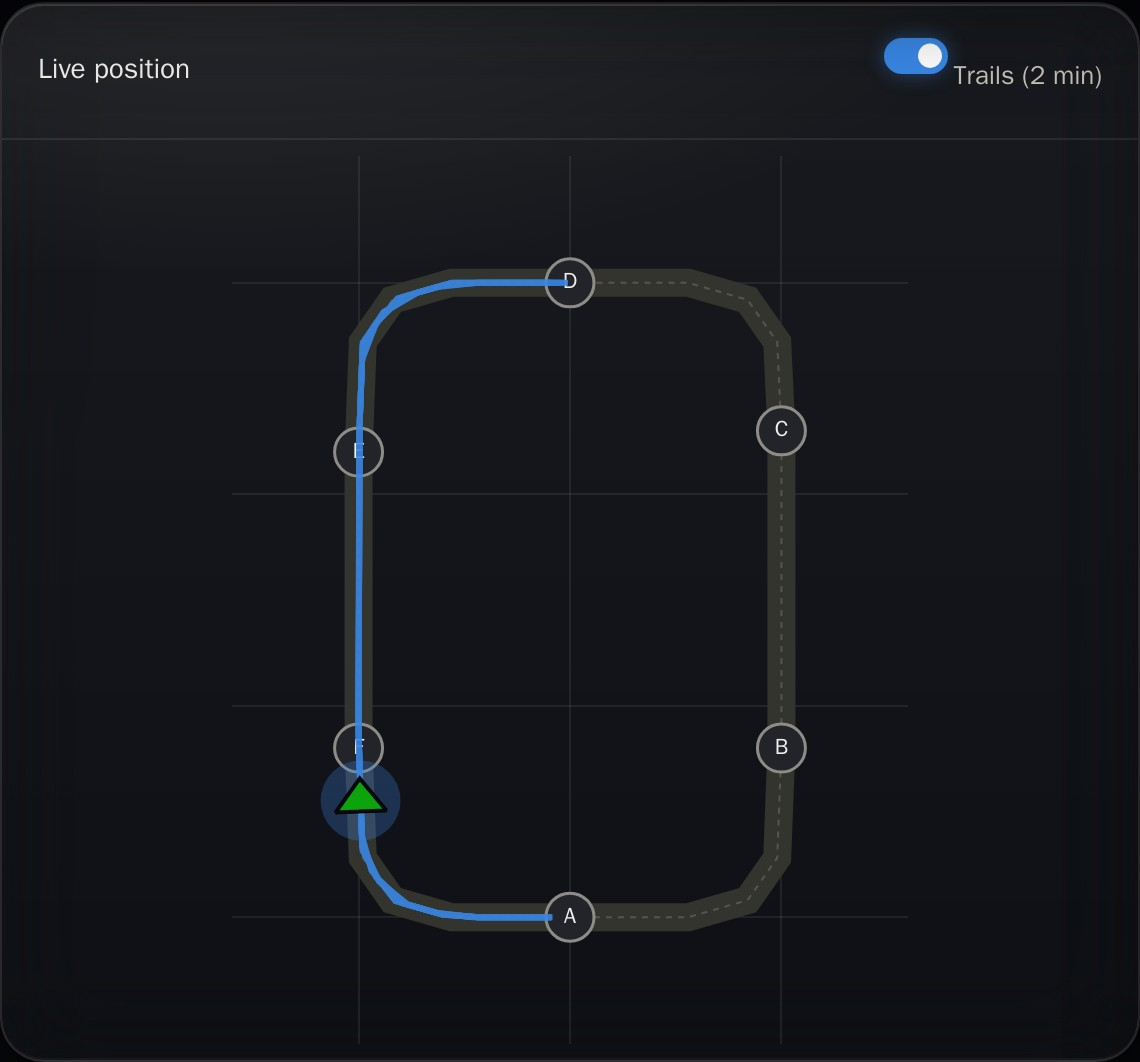
\includegraphics[width=\linewidth]{captures/tracking_map_proto.jpg}
  \caption{Prototype}
\end{subfigure}
\caption{Carte de suivi avec la position des véhicules et leurs traces}
\label{fig:tracking-map}
\end{figure}

\subsection{Suivi des déplacements}
L'option \emph{Trails (2 min)} trace le chemin parcouru par chaque véhicule pendant les deux dernières minutes. La
trace est interrompue à chaque nouveau trajet et lors d'un saut de position (retour de la voiture de démonstration au
départ), pour ne pas dessiner de lignes trompeuses. Le panneau \emph{Vehicles} liste les véhicules en plaçant d'abord
ceux qui posent problème (arrêtés, ligne perdue, en évitement), et le panneau \emph{Selected vehicle} détaille le
véhicule choisi : état, vitesse, batterie, distance à l'obstacle frontal et progression du trajet
(figure~\ref{fig:tracking-panels}).

\begin{figure}[H]
\centering
\begin{subfigure}[b]{0.49\linewidth}\centering
  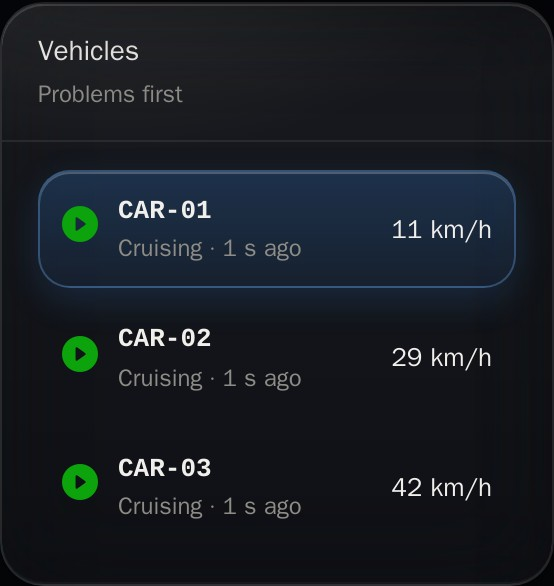
\includegraphics[width=\linewidth]{captures/tracking_vehicles.jpg}
  \caption{Liste des véhicules}
\end{subfigure}\hfill
\begin{subfigure}[b]{0.46\linewidth}\centering
  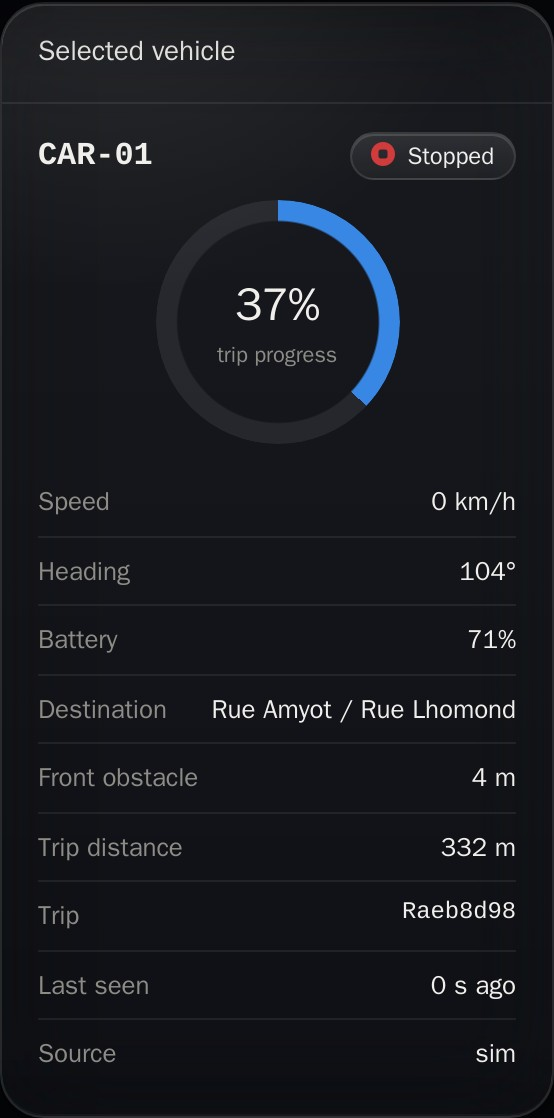
\includegraphics[width=\linewidth]{captures/tracking_selected.jpg}
  \caption{Véhicule sélectionné}
\end{subfigure}
\caption{Suivi des véhicules}
\label{fig:tracking-panels}
\end{figure}

\subsection{Historique des trajectoires}
Chaque trajet est enregistré avec ses points de trajectoire horodatés (position, vitesse, état), échantillonnés
chaque seconde. La table \emph{Trip history} présente les trajets récents : heure de départ, véhicule, itinéraire,
durée, distance et nombre d'obstacles rencontrés.

\subsection{Consultation des parcours précédents}
La sélection d'un trajet dans la table le rejoue sur une carte dédiée : le tracé complet apparaît, un curseur permet
de parcourir le trajet dans le temps et un graphique montre le profil de vitesse (figure~\ref{fig:tracking_history_real}).
Le dernier trajet terminé est sélectionné automatiquement à l'ouverture de la page.

\capture{tracking_history_real}{Historique des trajets et relecture d'un parcours précédent}

\subsection{Gestion des données de localisation}
Les positions courantes sont conservées dans le hub en mémoire (historique glissant pour les traces), alors que
les points de trajectoire des trajets sont écrits dans la base. En monde réel, les coordonnées sont des longitudes et
latitudes et les distances sont calculées en mètres ; dans le prototype, ce sont des coordonnées en centimètres sur le
plan de la piste. Un module de géométrie commun fournit les calculs de distance, de longueur de tracé et
d'interpolation dans les deux systèmes.

% =================================================================================================
\section{Page Camera : visualisation du flux vidéo}

\subsection{Intégration du flux vidéo de l'ESP32-CAM}
En mode prototype, la page affiche le flux de l'ESP32-CAM relayé par le serveur. Le panneau \emph{Connection}
indique l'état de la caméra, son adresse IP et la manière dont elle a été trouvée, la cadence, la résolution, le
détecteur utilisé et le nombre de points de passage reconnus ; il permet de saisir une adresse, de relancer la
recherche sur le réseau, de prendre un instantané et d'\textbf{enregistrer des images} pour enrichir le jeu de données
du prototype. Le panneau \emph{Camera settings} règle la résolution, la qualité JPEG, le flash, le retournement,
le miroir et la \textbf{rotation} de l'image (figure~\ref{fig:camera-proto-panels}).

\begin{figure}[H]
\centering
\begin{subfigure}[b]{0.49\linewidth}\centering
  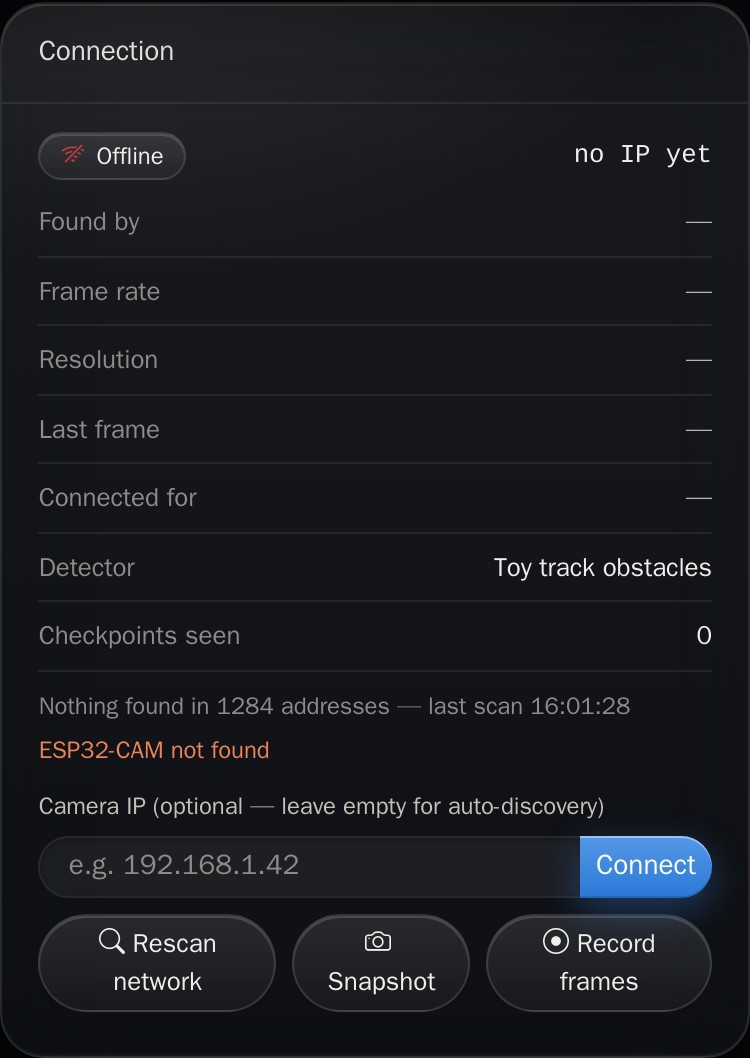
\includegraphics[width=\linewidth]{captures/camera_connection_proto.jpg}
  \caption{Connexion à l'ESP32-CAM}
\end{subfigure}\hfill
\begin{subfigure}[b]{0.49\linewidth}\centering
  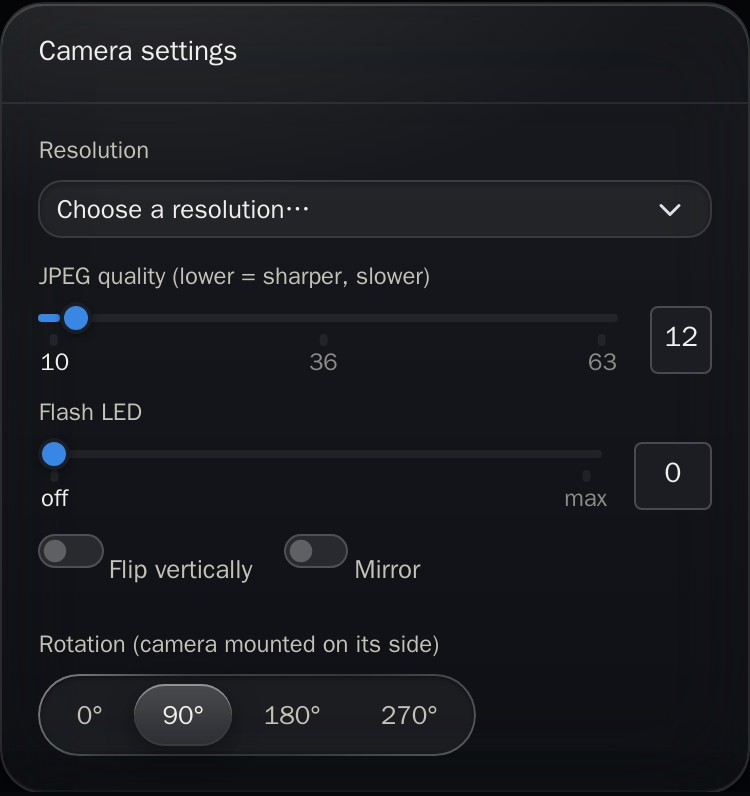
\includegraphics[width=\linewidth]{captures/camera_settings_proto.jpg}
  \caption{Réglages de la caméra}
\end{subfigure}
\caption{Panneaux de connexion et de réglage de l'ESP32-CAM}
\label{fig:camera-proto-panels}
\end{figure}

\subsection{Affichage des images en direct}
L'image est affichée dans un cadre au format de la caméra, surmonté d'un affichage tête haute : indicateur
\emph{LIVE}, cadence, résolution, état de la voiture, point de passage et itinéraire, heure. Un interrupteur
permet d'afficher ou de masquer les détections. Lorsque la caméra est hors ligne, une image d'attente explique la
situation (recherche en cours, dernière adresse connue).

\subsection{Intégration des résultats de l'intelligence artificielle}
Les détections du modèle sont dessinées directement sur l'image relayée : boîte, classe et confiance. En monde
réel, la couleur de la boîte correspond au niveau de gravité et l'étiquette indique aussi la distance estimée
(figure~\ref{fig:camera-ia}).

\begin{figure}[H]
\centering
\begin{subfigure}[b]{0.62\linewidth}\centering
  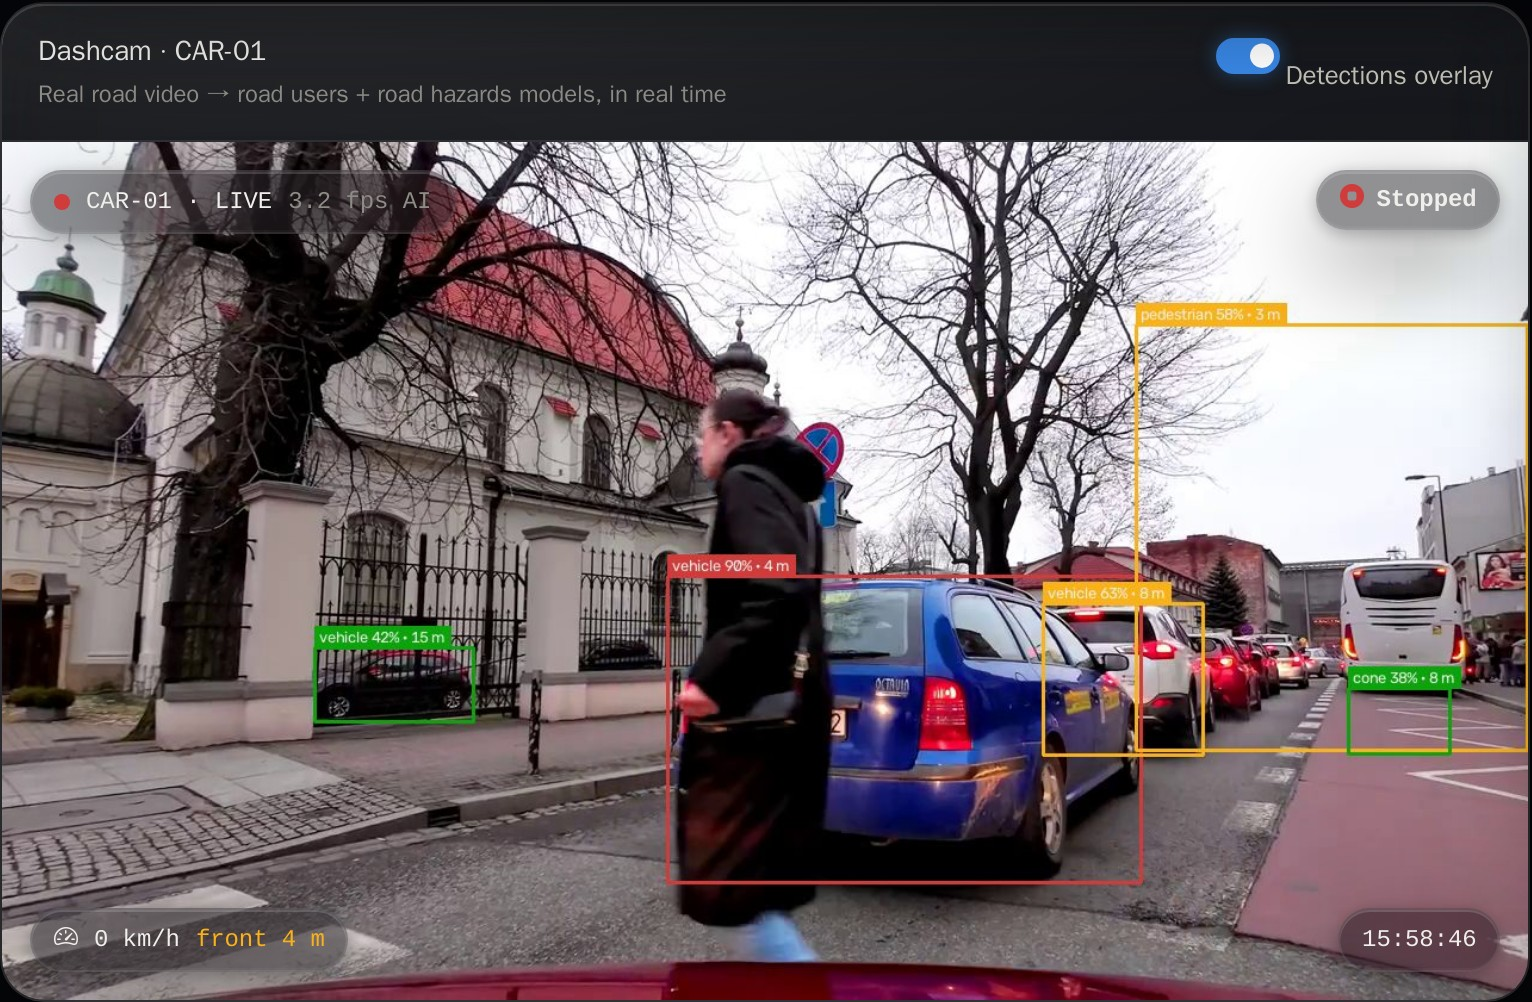
\includegraphics[width=\linewidth]{captures/camera_dashcam.jpg}
  \caption{Monde réel : caméra embarquée de CAR-01}
\end{subfigure}\hfill
\begin{subfigure}[b]{0.36\linewidth}\centering
  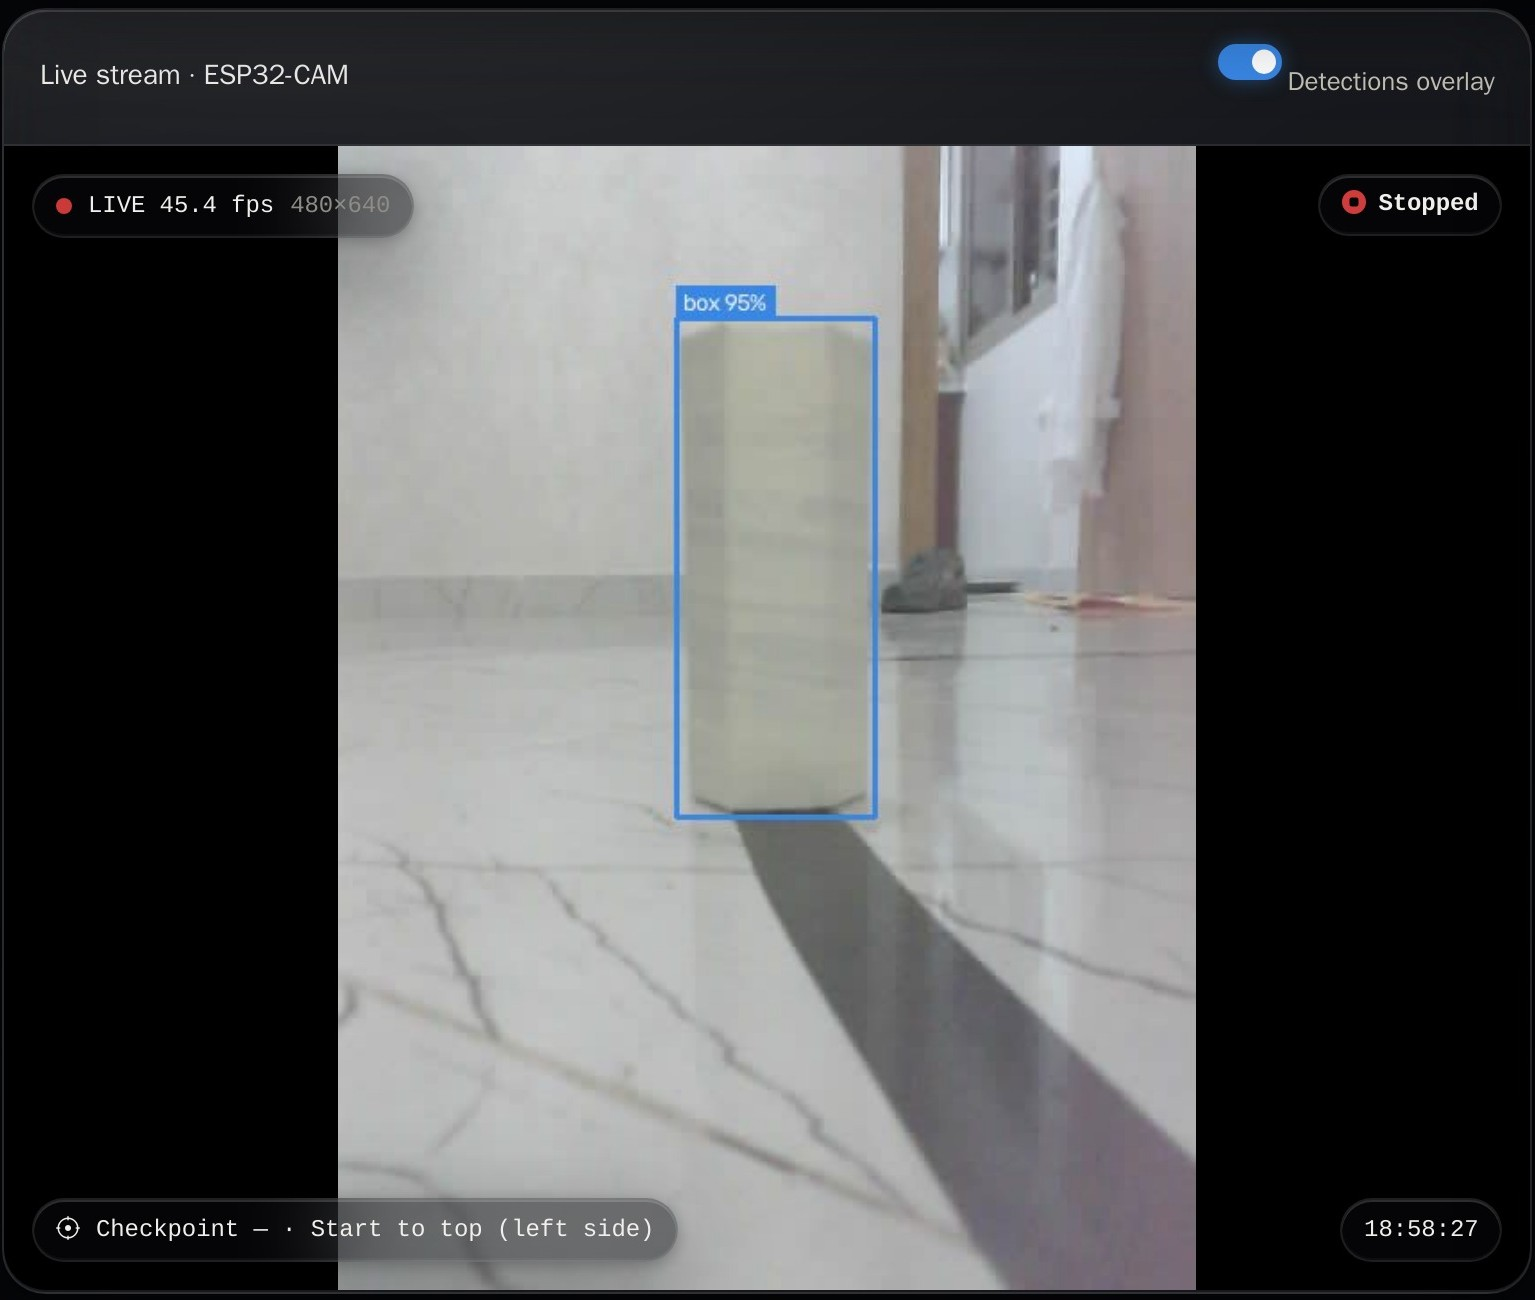
\includegraphics[width=\linewidth]{captures/camera_proto.jpg}
  \caption{Prototype : ESP32-CAM}
\end{subfigure}
\caption{Flux vidéo avec les prédictions des modèles affichées}
\label{fig:camera-ia}
\end{figure}

\subsection{Visualisation des détections sur les images}
Sous la vidéo, le panneau \emph{Live detections} liste les dernières détections (une entrée par classe et par
demi-seconde au plus) avec la confiance, la distance estimée et la position par rapport à la trajectoire ; le
panneau \emph{Models} rappelle les modèles chargés et leur temps d'exécution (figure~\ref{fig:camera-lists}). En mode
prototype, le panneau \emph{Snapshots} rassemble les instantanés enregistrés.

\begin{figure}[H]
\centering
\begin{subfigure}[b]{0.56\linewidth}\centering
  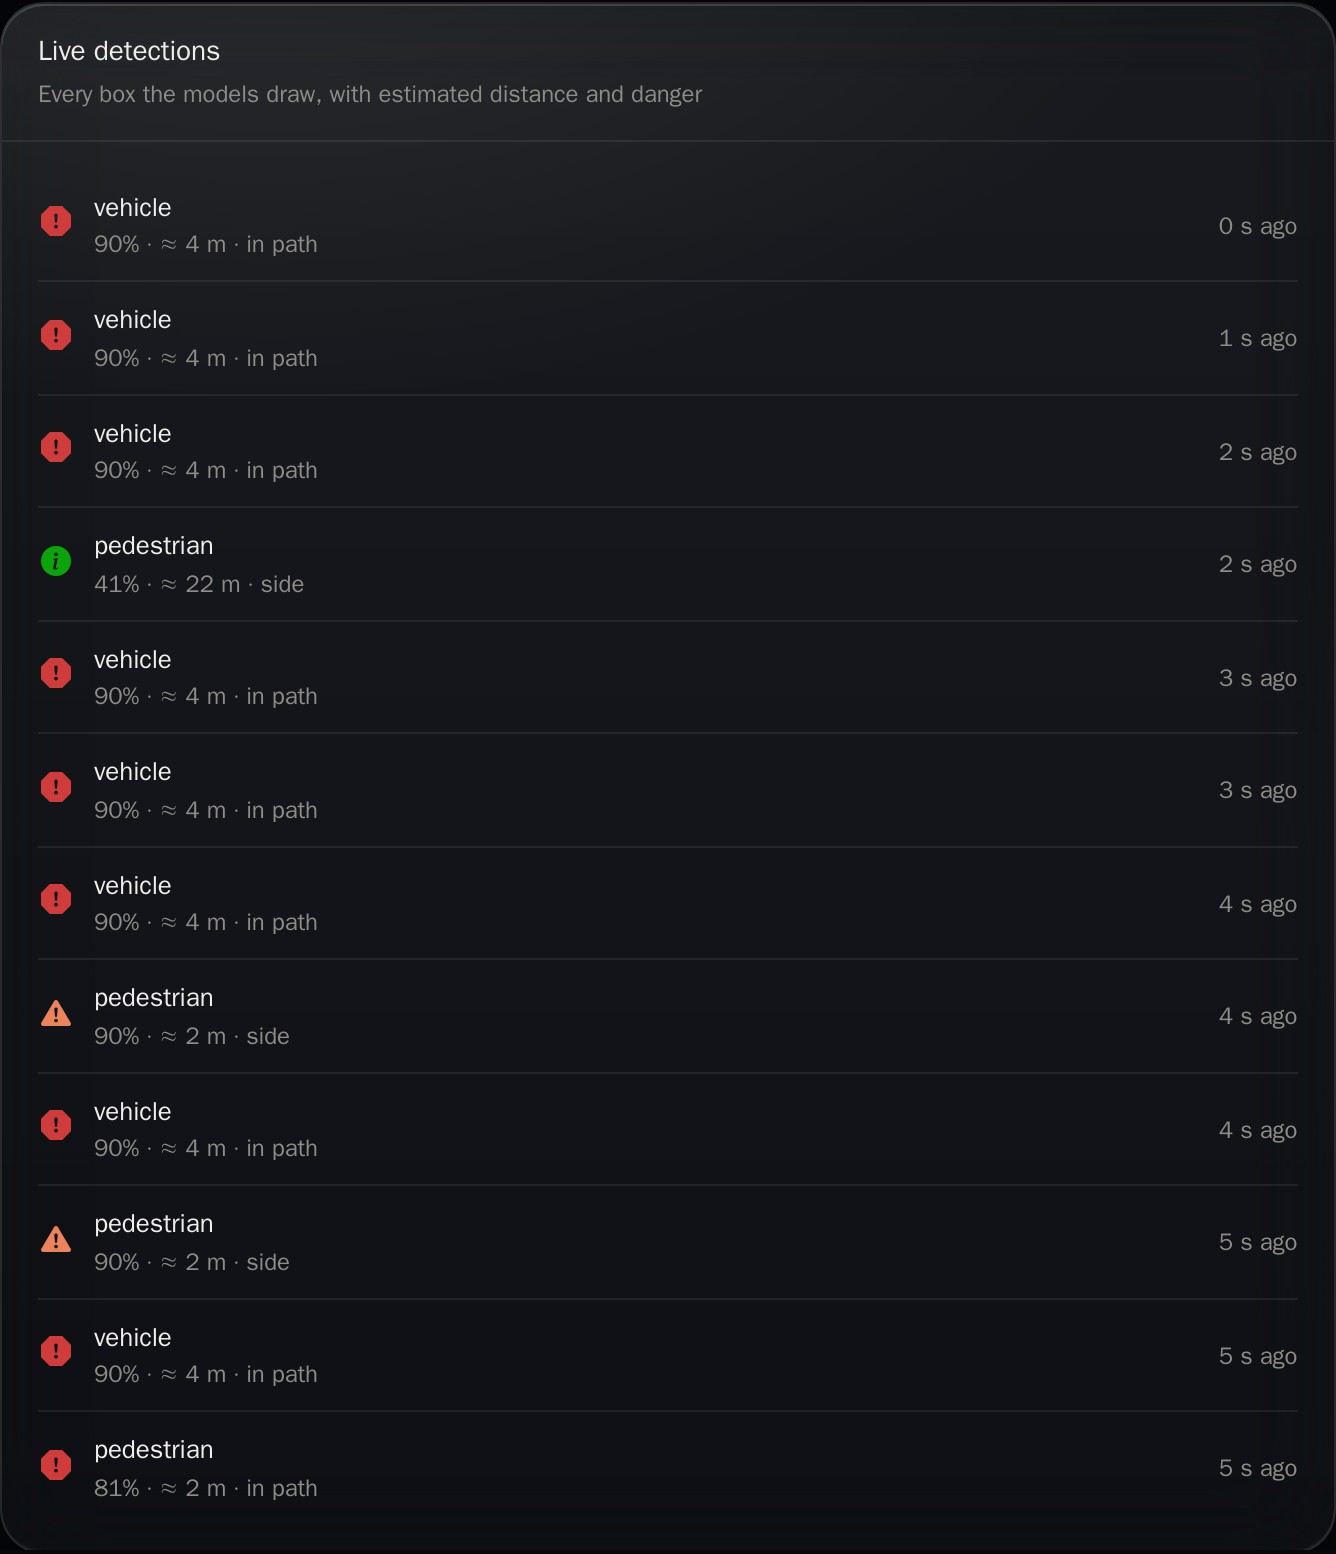
\includegraphics[width=\linewidth]{captures/camera_detections_real.jpg}
  \caption{Dernières détections}
\end{subfigure}\hfill
\begin{subfigure}[b]{0.41\linewidth}\centering
  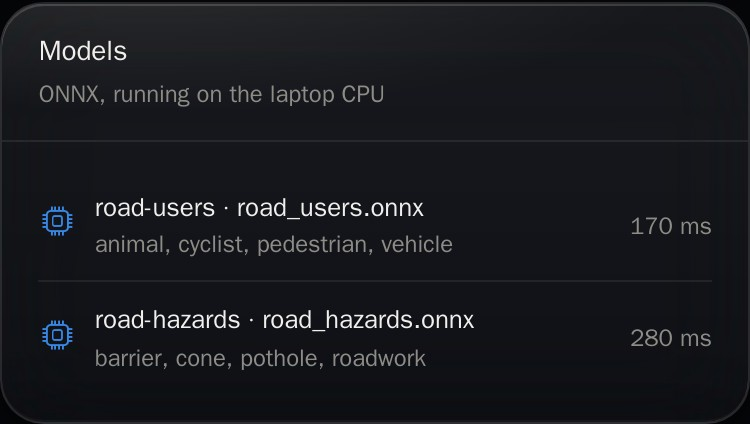
\includegraphics[width=\linewidth]{captures/camera_models_real.jpg}

  \vspace{0.2cm}
  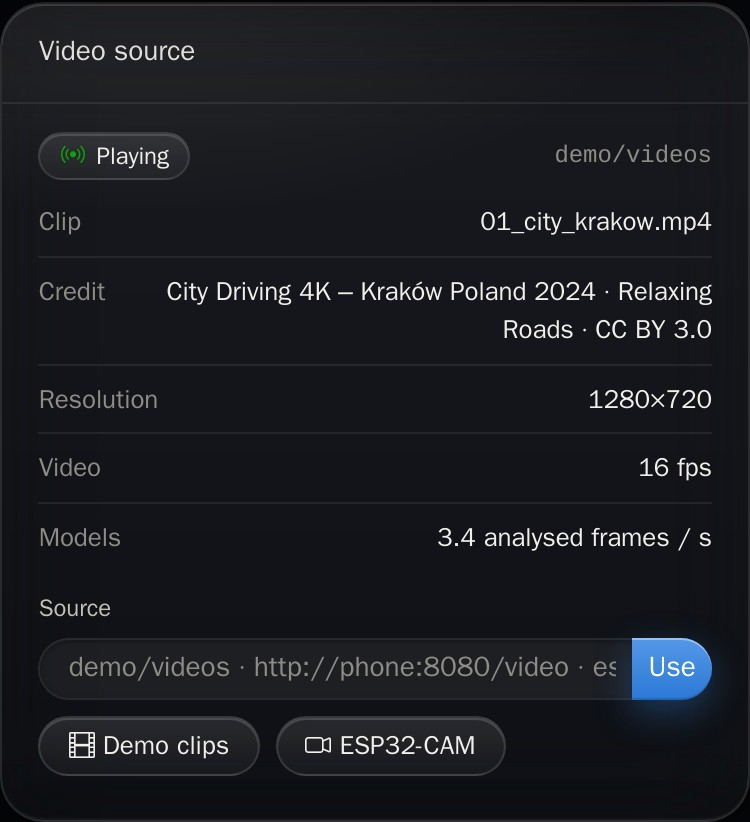
\includegraphics[width=\linewidth]{captures/camera_source_real.jpg}
  \caption{Modèles chargés et source vidéo}
\end{subfigure}
\caption{Détections, modèles et source de la page Camera (monde réel)}
\label{fig:camera-lists}
\end{figure}

\subsection{Comparaison entre les vues Real World et Prototype}
Les deux vues partagent la même logique (relais, détection, affichage tête haute, liste des détections) mais
diffèrent par leur source et leur exploitation. En monde réel, la source est une vidéo de route choisie dans le
panneau \emph{Video source} (clips de démonstration, flux réseau ou ESP32-CAM) et les détections pilotent les
réactions de CAR-01 et la carte des obstacles. En prototype, la source est l'ESP32-CAM de la voiture ; les détections
alimentent la liste des obstacles de la piste et l'état de la voiture.

% =================================================================================================
\section{Page Route Planner : planification des itinéraires}

\subsection{Présentation de l'interface cartographique}
La page \emph{Route planner} associe un formulaire, une carte et une liste d'itinéraires proposés
(figure~\ref{fig:planner_form_real}). La carte affiche le réseau, les obstacles ouverts et, si l'option \emph{Risk
layer} est active, les tronçons à risque colorés selon leur niveau.

\capture[0.6]{planner_form_real}{Formulaire de planification d'itinéraire}

\subsection{Sélection des points de départ et d'arrivée}
Le départ et la destination se choisissent dans des listes d'intersections nommées d'après leurs rues (monde réel)
ou parmi les points de passage de la piste (prototype). Des valeurs par défaut pertinentes sont proposées : deux
intersections éloignées dans le monde réel, le départ et l'arrivée d'une trajectoire de la piste dans le prototype.

\subsection{Représentation des obstacles sur la carte}
Les obstacles ouverts sont représentés par des marqueurs colorés selon leur niveau de gravité ; les tronçons dont le
risque dépasse un seuil sont surlignés en orange (élevé) ou en rouge (critique). Les seuils diffèrent entre les deux
environnements, car la piste, très courte, accumule le risque plus vite.

\subsection{Calcul des itinéraires possibles}
Le réseau est représenté par un graphe : les nœuds sont les intersections (ou points de passage), les arêtes les
tronçons, avec leur géométrie et leur longueur. Les itinéraires sont calculés par l'algorithme de plus court chemin
de Dijkstra~\cite{dijkstra1959} de la bibliothèque NetworkX~\cite{networkx}, avec un coût qui combine distance et
risque.

\subsection{Prise en compte de la distance, des obstacles et de leur gravité}
Chaque tronçon reçoit un \textbf{risque} calculé à partir de l'historique des obstacles qui s'y trouvent :
\begin{equation}
  \text{risque}(e) = \sum_{o \in e} \frac{\text{score}_o}{100} \times w_{\text{statut}} \times
  0{,}5^{\,\text{âge}_o / T_{1/2}}
\end{equation}
Les obstacles graves comptent davantage, les obstacles anciens s'effacent progressivement (demi-vie $T_{1/2}$ de
7 jours dans le monde réel, 2 jours sur la piste), les obstacles résolus ne comptent plus que pour 30\,\% et les faux
positifs sont ignorés. Le coût d'un tronçon est alors :
\begin{equation}
  \text{coût}(e) = \text{longueur}(e) + \alpha \times U \times \text{risque}(e)
\end{equation}
où $U$ exprime la distance qu'« équivaut » une unité de risque (150 m dans le monde réel, 60 cm sur la piste) et
$\alpha$ la priorité choisie par l'opérateur avec le curseur : $\alpha = 0$ donne le plus court chemin, une grande
valeur l'itinéraire le plus sûr.

\subsection{Sélection et affichage de l'itinéraire recommandé}
Trois itinéraires sont calculés : \emph{Recommended} (priorité choisie), \emph{Shortest} ($\alpha = 0$) et
\emph{Safest} ($\alpha = 8$). Lorsque deux d'entre eux coïncident, ils sont fusionnés. L'itinéraire recommandé est
tracé sur la carte avec les obstacles (figure~\ref{fig:planner-route}) ; une phrase résume le compromis, par exemple
« +43 \% de distance par rapport au plus court, 50 \% de risque en moins, évite 35 obstacles ouverts ».

\begin{figure}[H]
\centering
\begin{subfigure}[b]{0.58\linewidth}\centering
  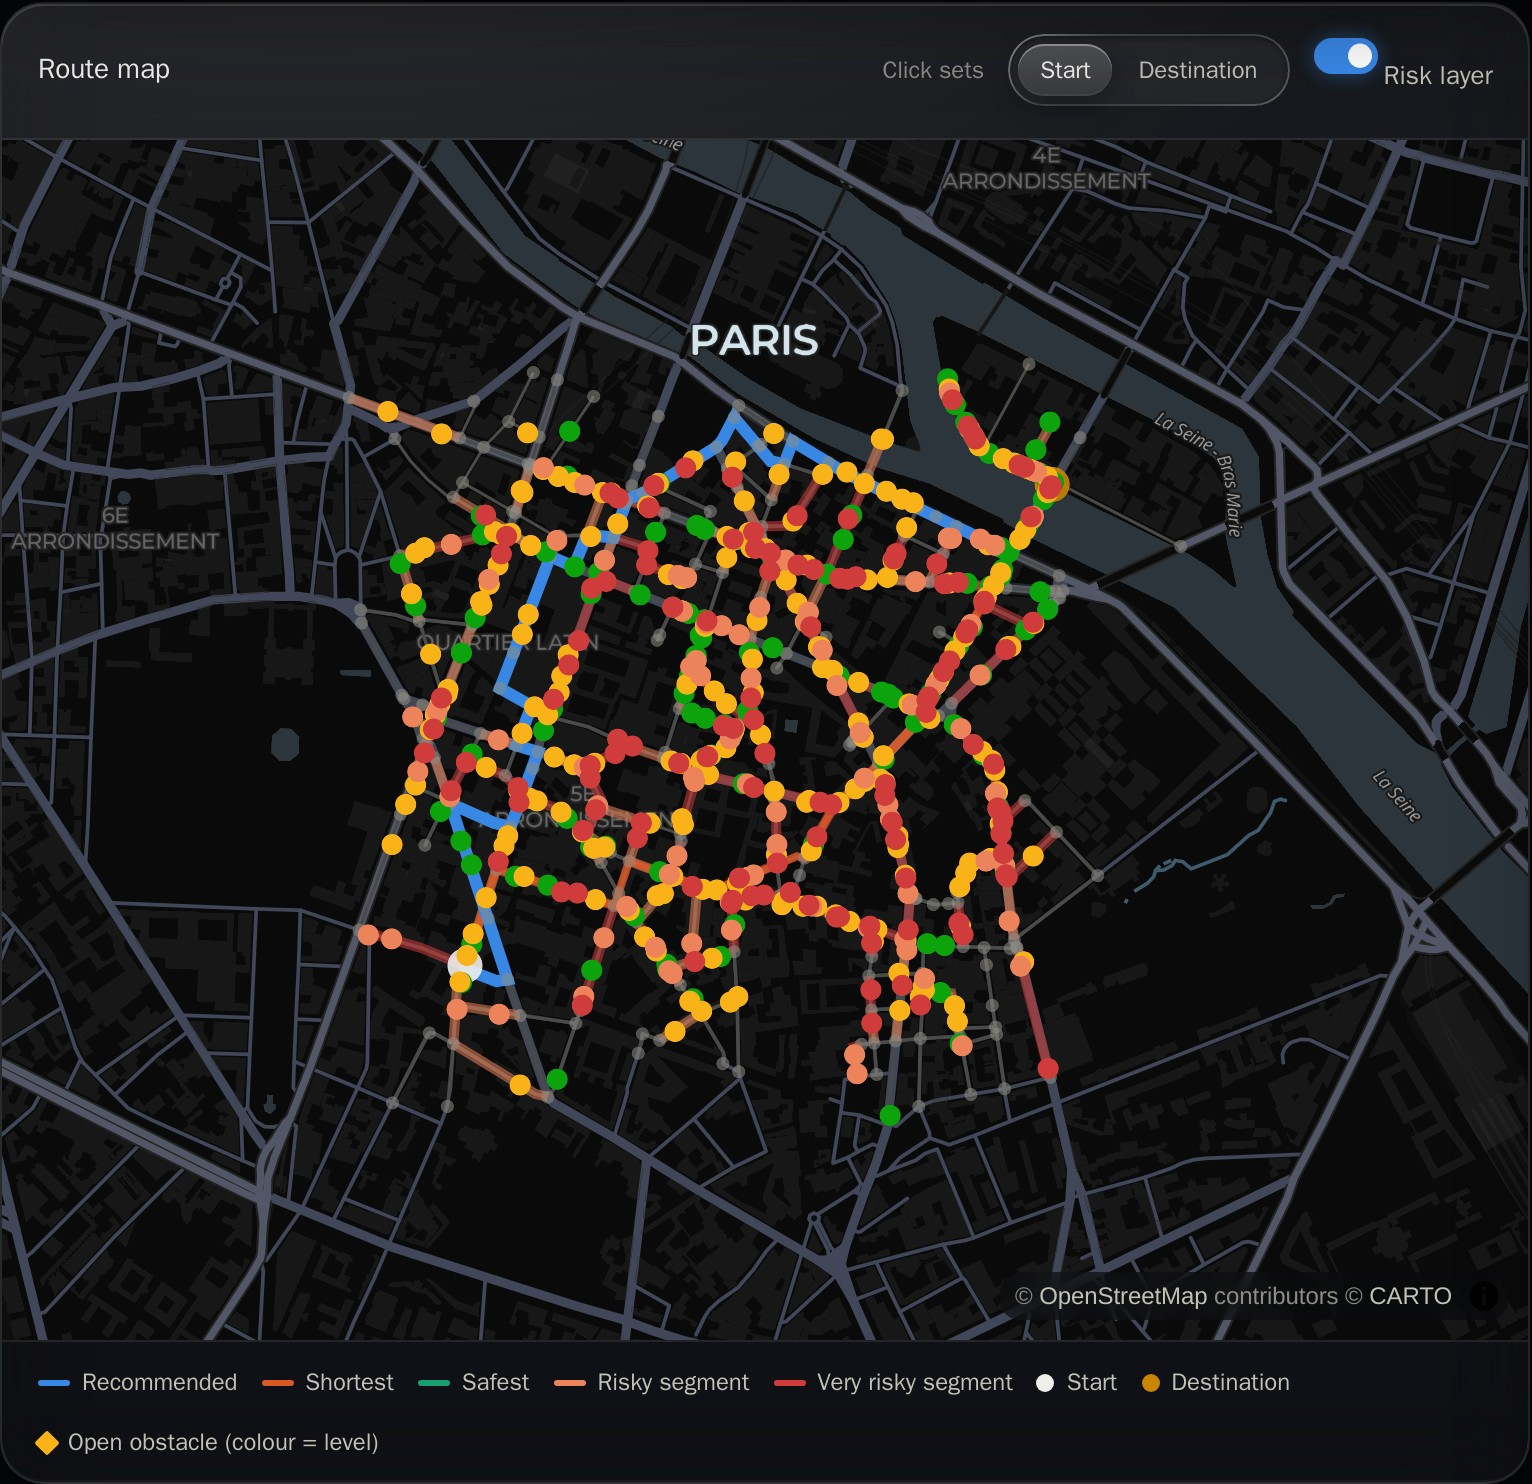
\includegraphics[width=\linewidth]{captures/planner_map_real.jpg}
  \caption{Carte avec l'itinéraire proposé et les obstacles}
\end{subfigure}\hfill
\begin{subfigure}[b]{0.4\linewidth}\centering
  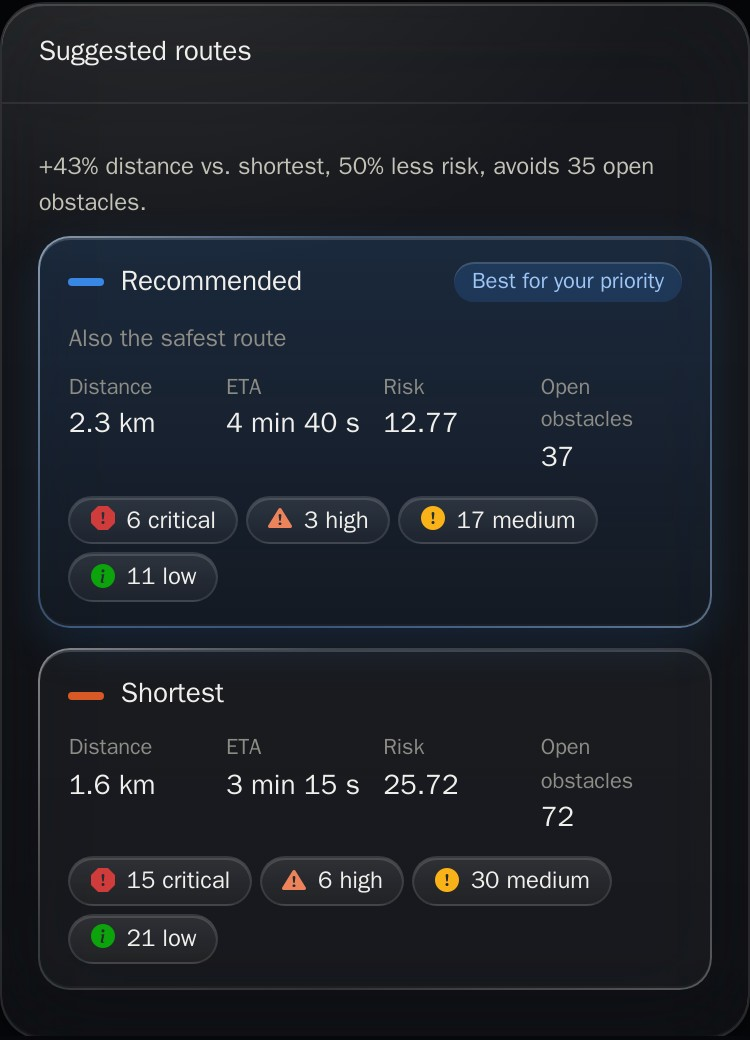
\includegraphics[width=\linewidth]{captures/planner_routes_real.jpg}
  \caption{Itinéraires proposés}
\end{subfigure}
\caption{Itinéraire recommandé, obstacles et tronçons à risque}
\label{fig:planner-route}
\end{figure}

\subsection{Comparaison des itinéraires proposés}
Chaque itinéraire est présenté sur une carte de synthèse avec sa distance, sa durée estimée, son risque cumulé et le
nombre d'obstacles ouverts sur son parcours, répartis par niveau. L'opérateur compare ainsi d'un coup d'œil le gain
de sécurité et le coût en distance. En mode prototype, la page ajoute le classement des \textbf{trajectoires
manuelles} de la piste selon le même coût et un \textbf{éditeur de piste} : positions des points de passage en
centimètres, tronçons, trajectoires, et téléchargement des marqueurs ArUco à imprimer
(figure~\ref{fig:planner-proto}).

\begin{figure}[H]
\centering
\begin{subfigure}[b]{0.49\linewidth}\centering
  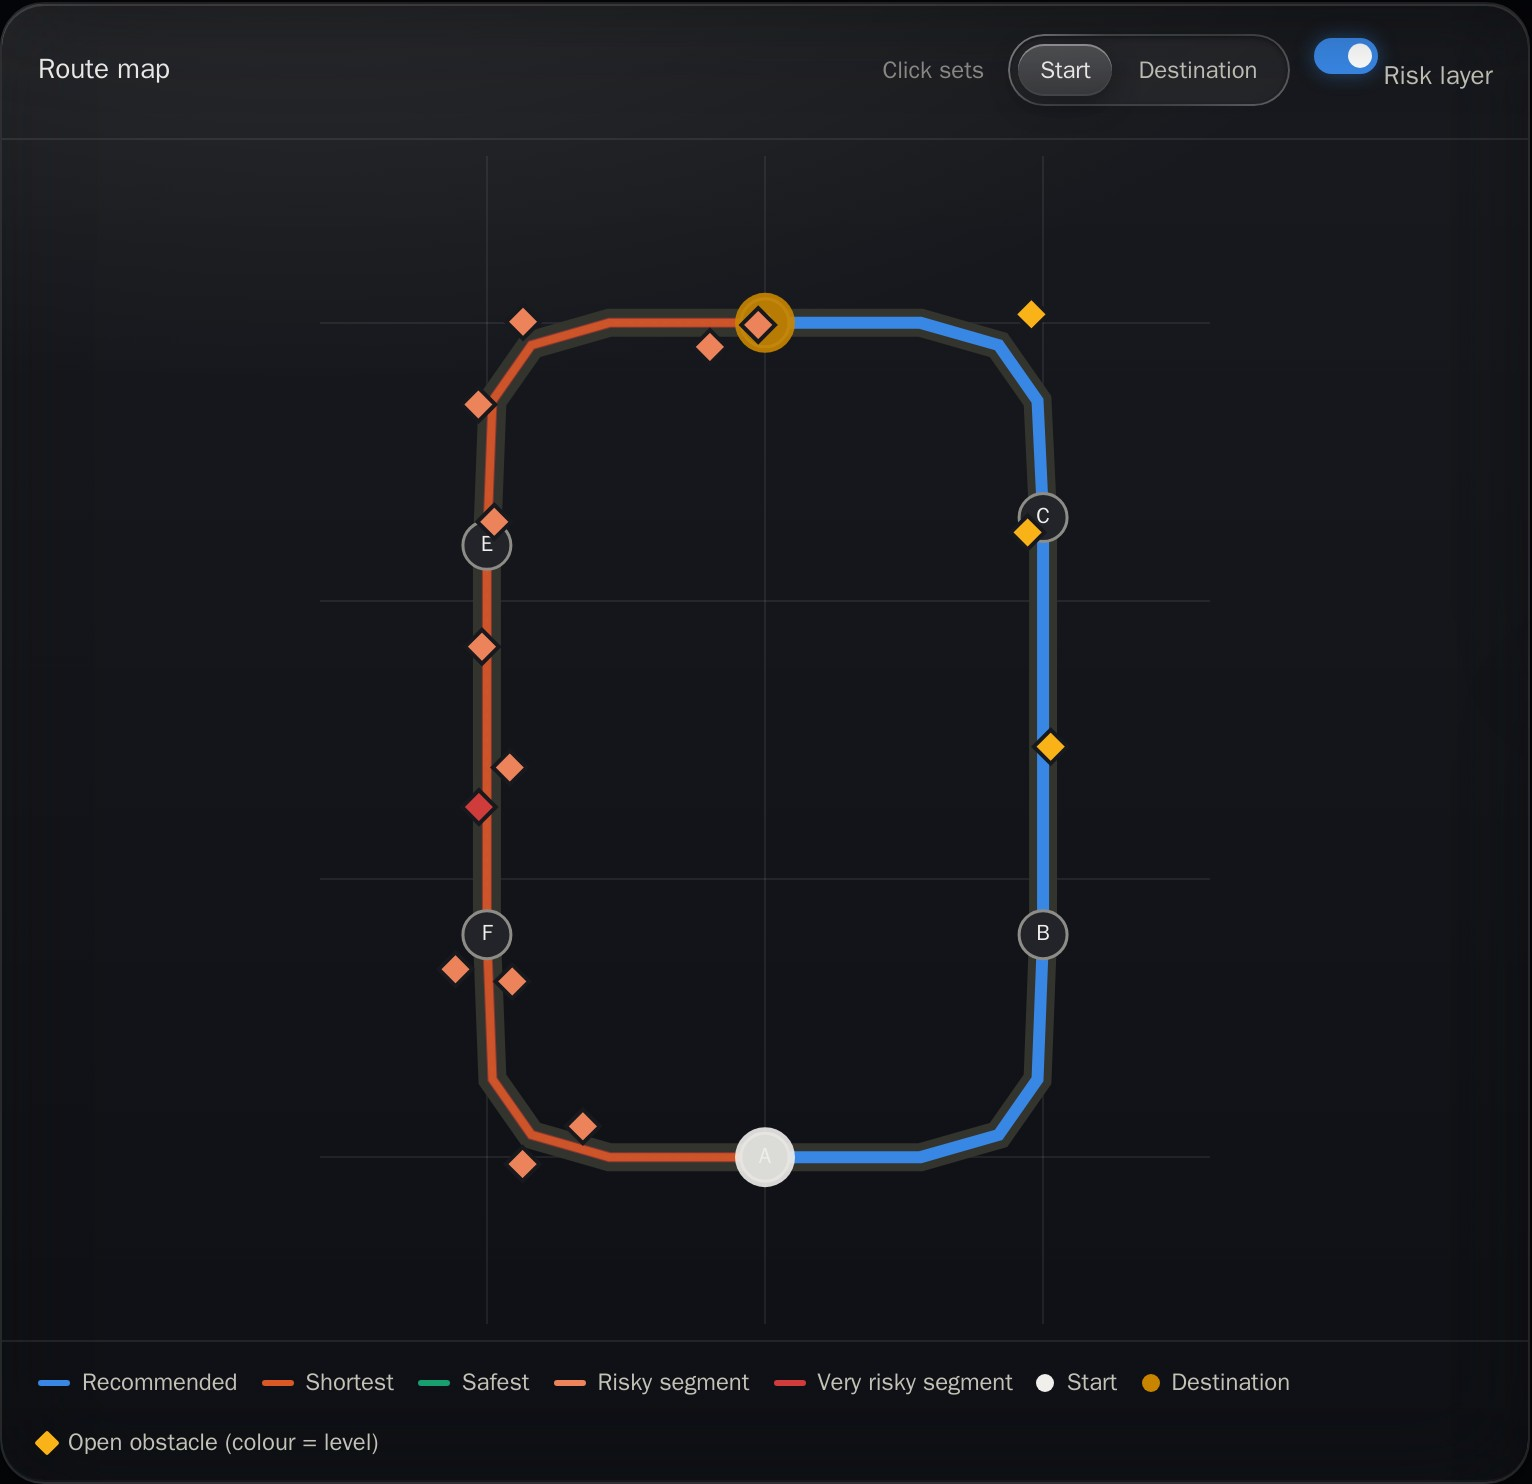
\includegraphics[width=\linewidth]{captures/planner_map_proto.jpg}
  \caption{Carte de la piste}
\end{subfigure}\hfill
\begin{subfigure}[b]{0.49\linewidth}\centering
  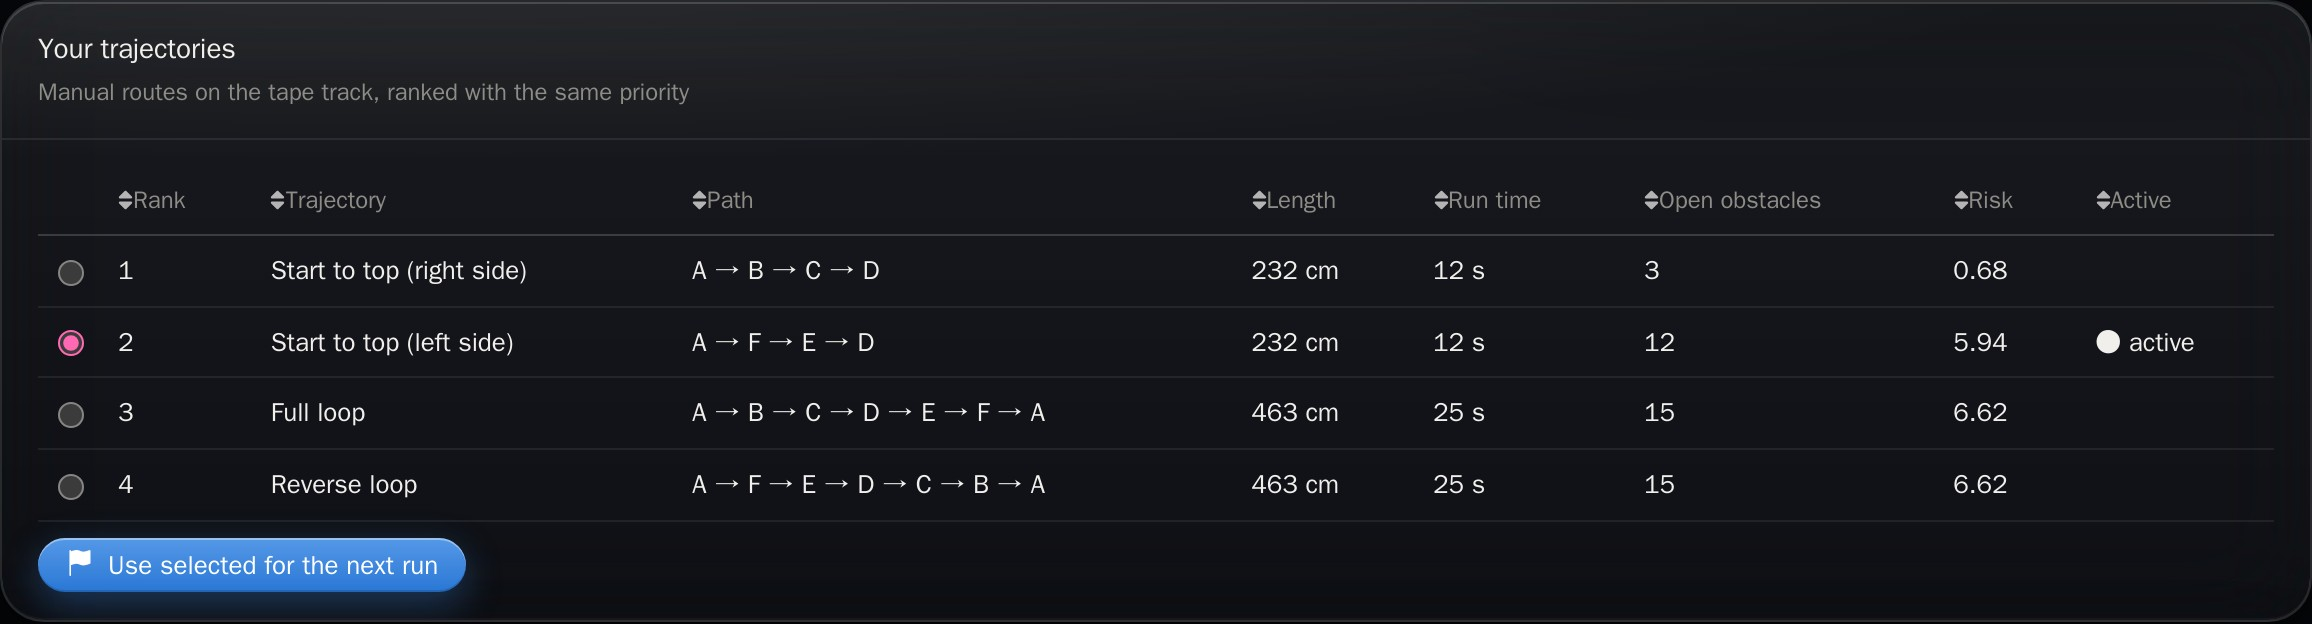
\includegraphics[width=\linewidth]{captures/planner_trajectories_proto.jpg}
  \caption{Trajectoires classées selon la priorité}
\end{subfigure}

\vspace{0.2cm}
\begin{subfigure}[b]{\linewidth}\centering
  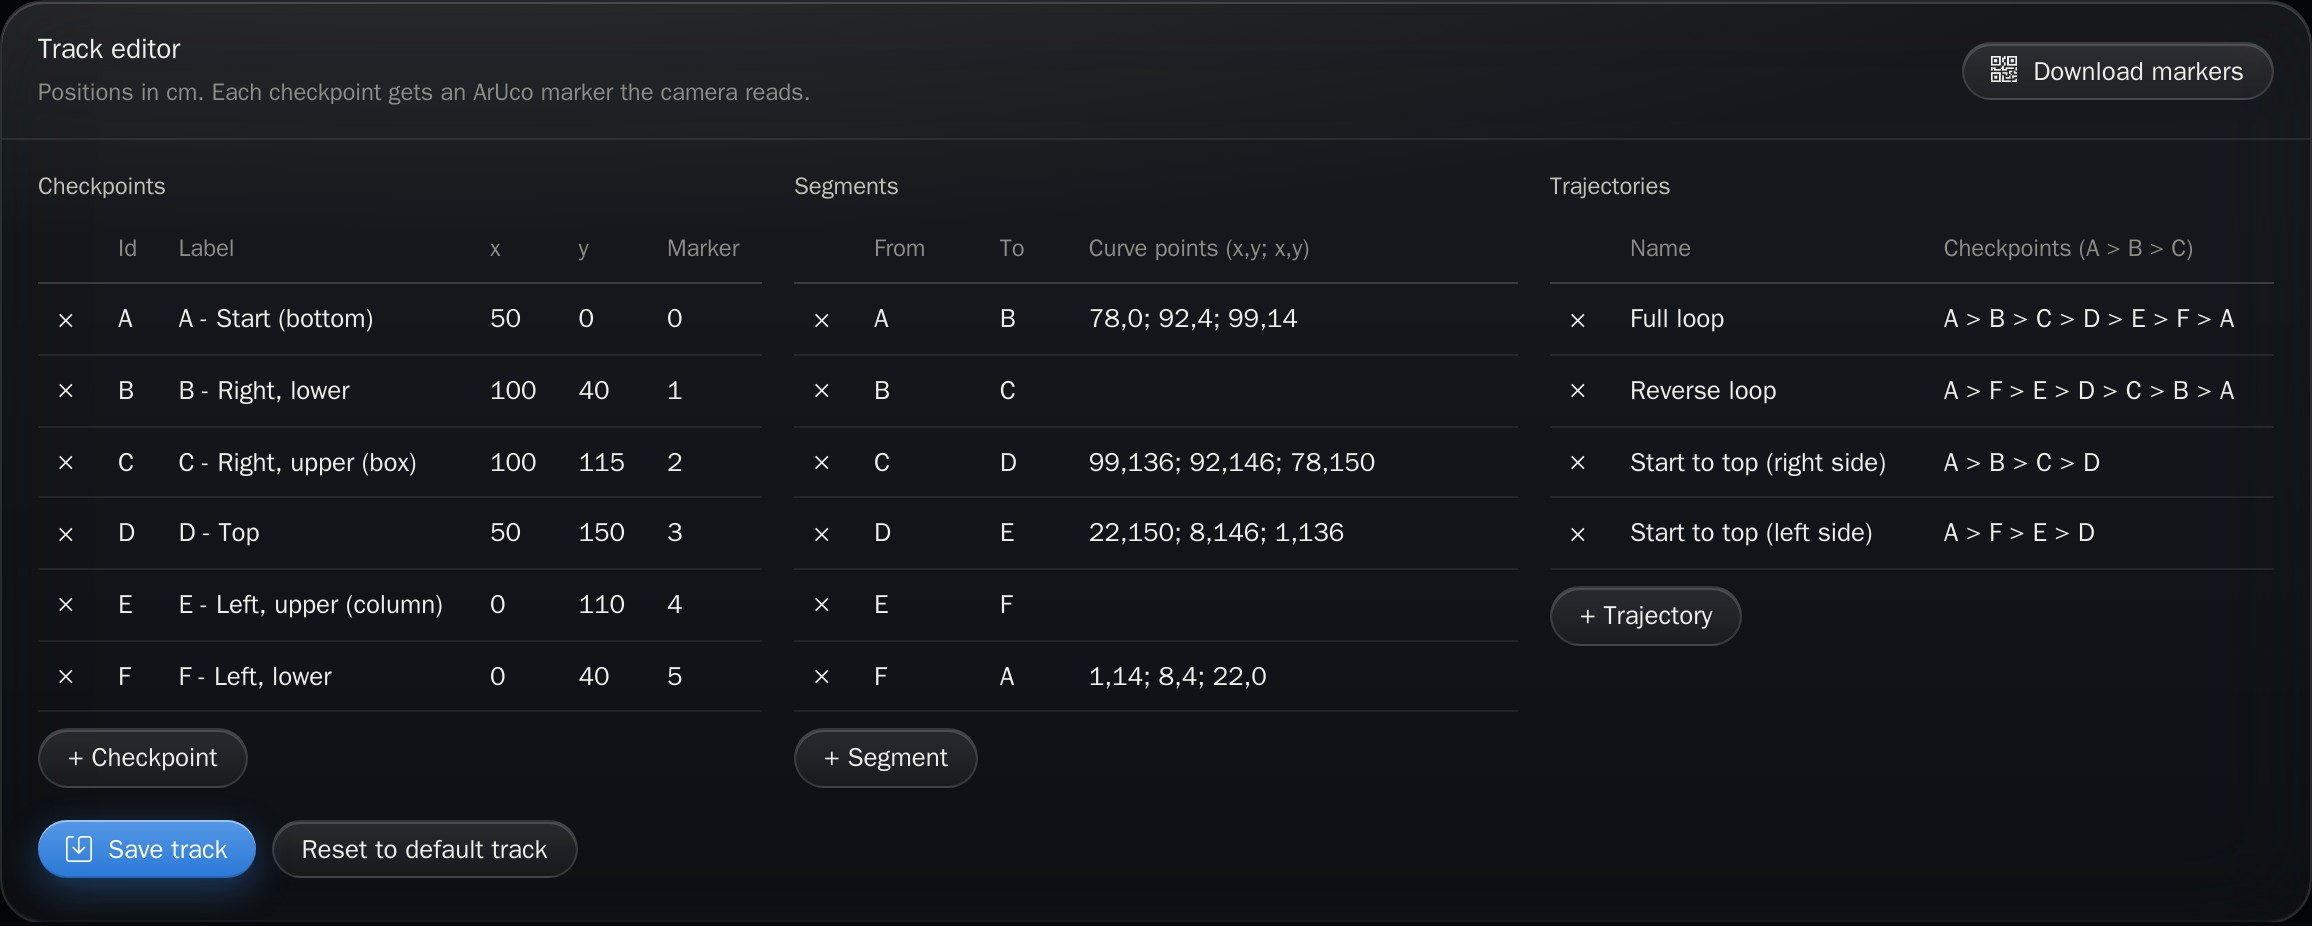
\includegraphics[width=0.8\linewidth]{captures/planner_editor_proto.jpg}
  \caption{Éditeur de piste}
\end{subfigure}
\caption{Planification dans l'environnement prototype}
\label{fig:planner-proto}
\end{figure}

% =================================================================================================
\section{Page Obstacles : gestion et priorisation des anomalies}

La page \emph{Obstacles} est le centre de gestion des anomalies. Elle présente, en haut, une barre de filtres et des
indicateurs, puis la file de priorité, le détail de l'obstacle sélectionné, une carte, une répartition par classe et
par niveau, et une explication du calcul de la priorité (figure~\ref{fig:obstacles_queue}).

\capture{obstacles_queue}{Liste des anomalies détectées, triées par priorité}

\subsection{Affichage des obstacles détectés}
La file de priorité est une table paginée qui présente pour chaque obstacle : son niveau, son score, la classe, la
confiance, la distance estimée, sa position sur la trajectoire ou sur le côté, le nombre d'observations, la date de la
dernière observation, le statut et le véhicule qui l'a détecté. Les obstacles vus plusieurs fois n'apparaissent
qu'une fois, avec leur compteur d'observations.

\subsection{Identification des nids-de-poule et autres anomalies}
Les anomalies proviennent de deux sources : les détections réelles des modèles (caméra embarquée de CAR-01 et
ESP32-CAM du prototype), accompagnées d'un instantané annoté, et les rencontres produites par le simulateur pour
les autres véhicules de la flotte, signalées comme simulées. Le détail de l'obstacle précise sa source.

\subsection{Classification des obstacles par catégorie}
Chaque obstacle porte l'une des classes du vocabulaire commun : piéton, cycliste, animal, véhicule, nid-de-poule,
cône, barrière, panneau de chantier, débris, et, pour le prototype, colonne et boîte. Un filtre permet de n'afficher
que certaines classes, et le graphique \emph{By object and level} montre leur répartition
(figure~\ref{fig:obstacles-repartition}).

\begin{figure}[H]
\centering
\begin{subfigure}[b]{0.49\linewidth}\centering
  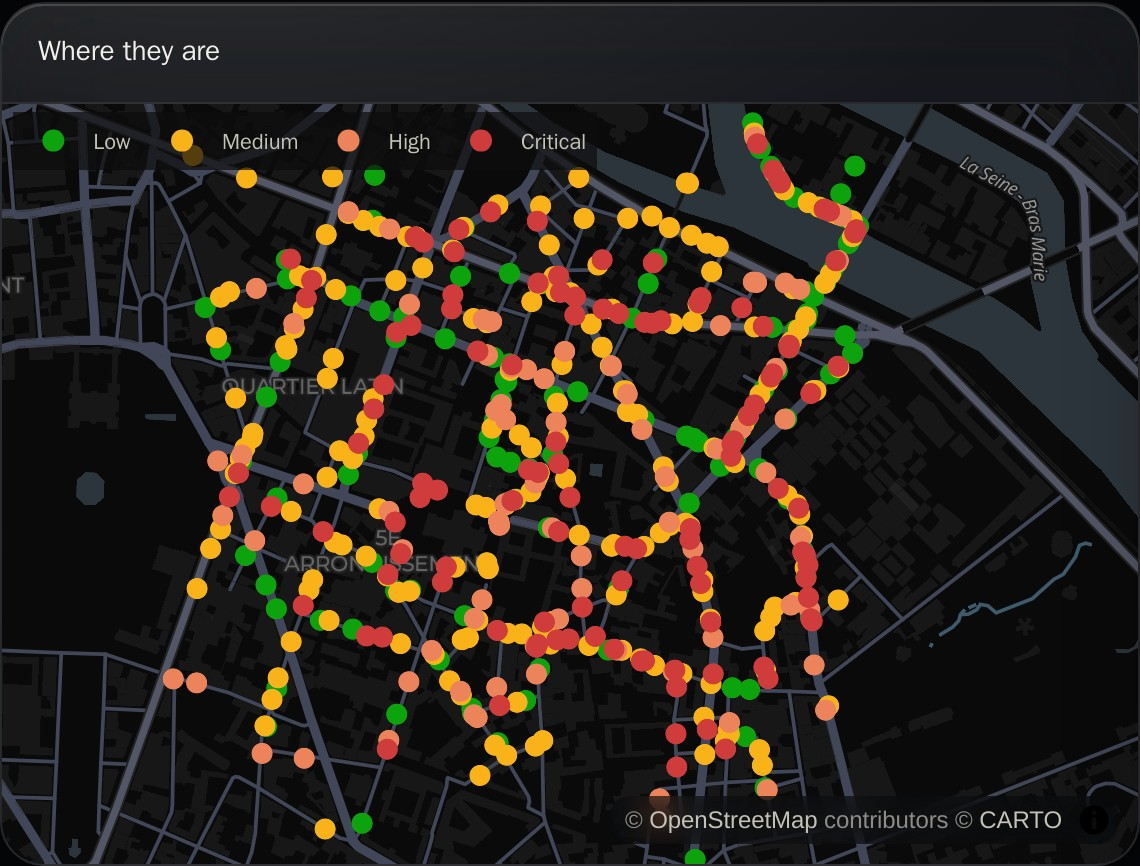
\includegraphics[width=\linewidth]{captures/obstacles_map.jpg}
  \caption{Localisation des obstacles par niveau}
\end{subfigure}\hfill
\begin{subfigure}[b]{0.49\linewidth}\centering
  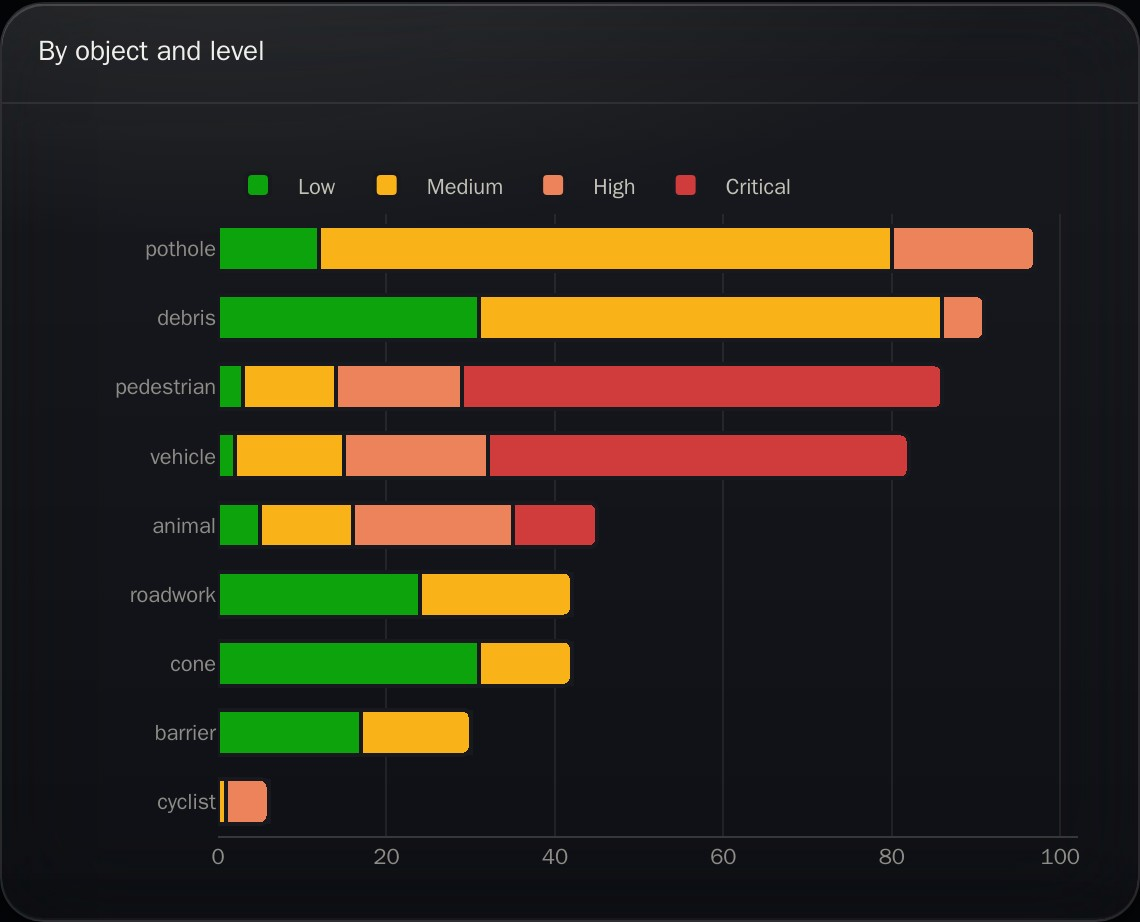
\includegraphics[width=\linewidth]{captures/obstacles_bars.jpg}
  \caption{Répartition par classe et par niveau}
\end{subfigure}
\caption{Carte et répartition des obstacles}
\label{fig:obstacles-repartition}
\end{figure}

\subsection{Évaluation de la gravité}
La gravité de chaque obstacle est le score explicable présenté au chapitre~3, qui combine le poids de danger de la
classe, la proximité, la confiance et la présence sur la trajectoire. Le panneau \emph{How priority is computed}
rappelle la formule et les seuils des niveaux à l'opérateur, et le détail de l'obstacle en montre chaque composante
(figure~\ref{fig:obstacles-gravite}).

\begin{figure}[H]
\centering
\begin{subfigure}[b]{0.32\linewidth}\centering
  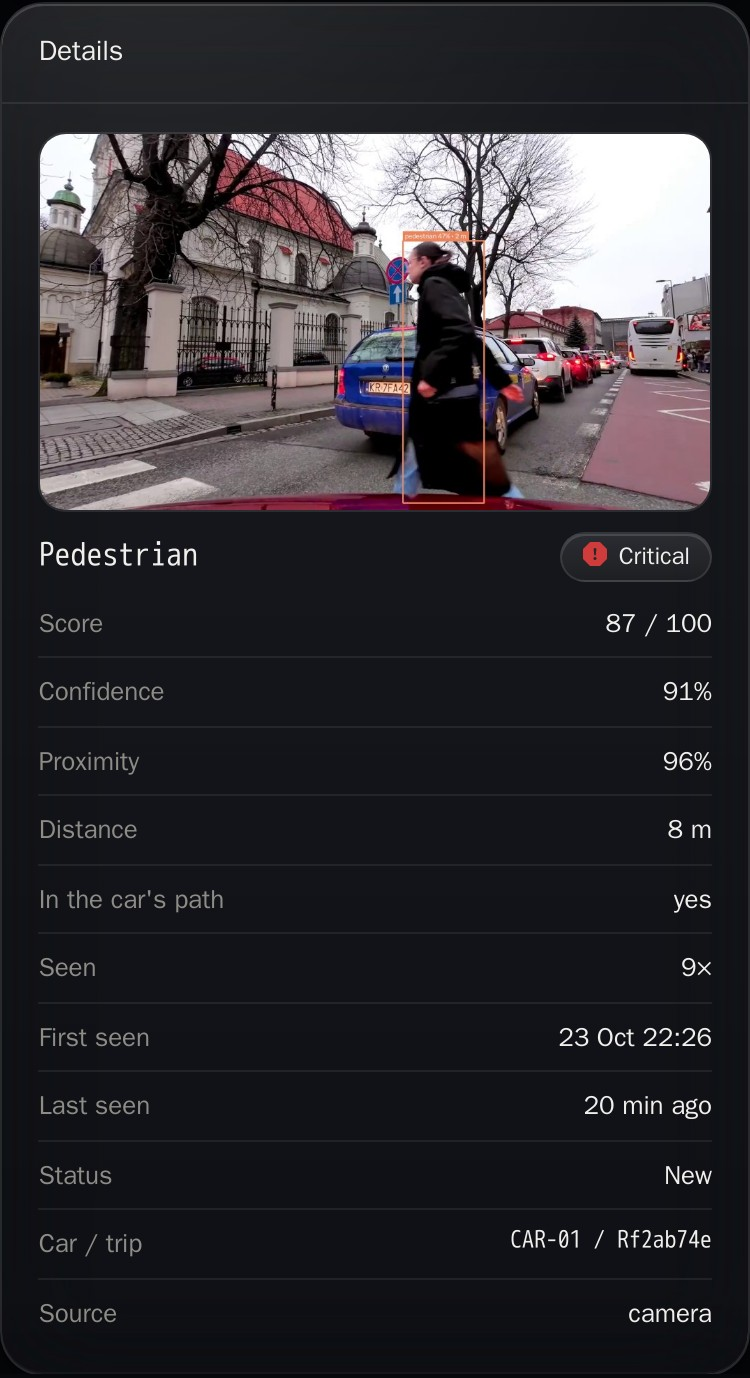
\includegraphics[width=\linewidth]{captures/obstacles_details_car01.jpg}
  \caption{Piéton sur la trajectoire : critique}
\end{subfigure}\hfill
\begin{subfigure}[b]{0.32\linewidth}\centering
  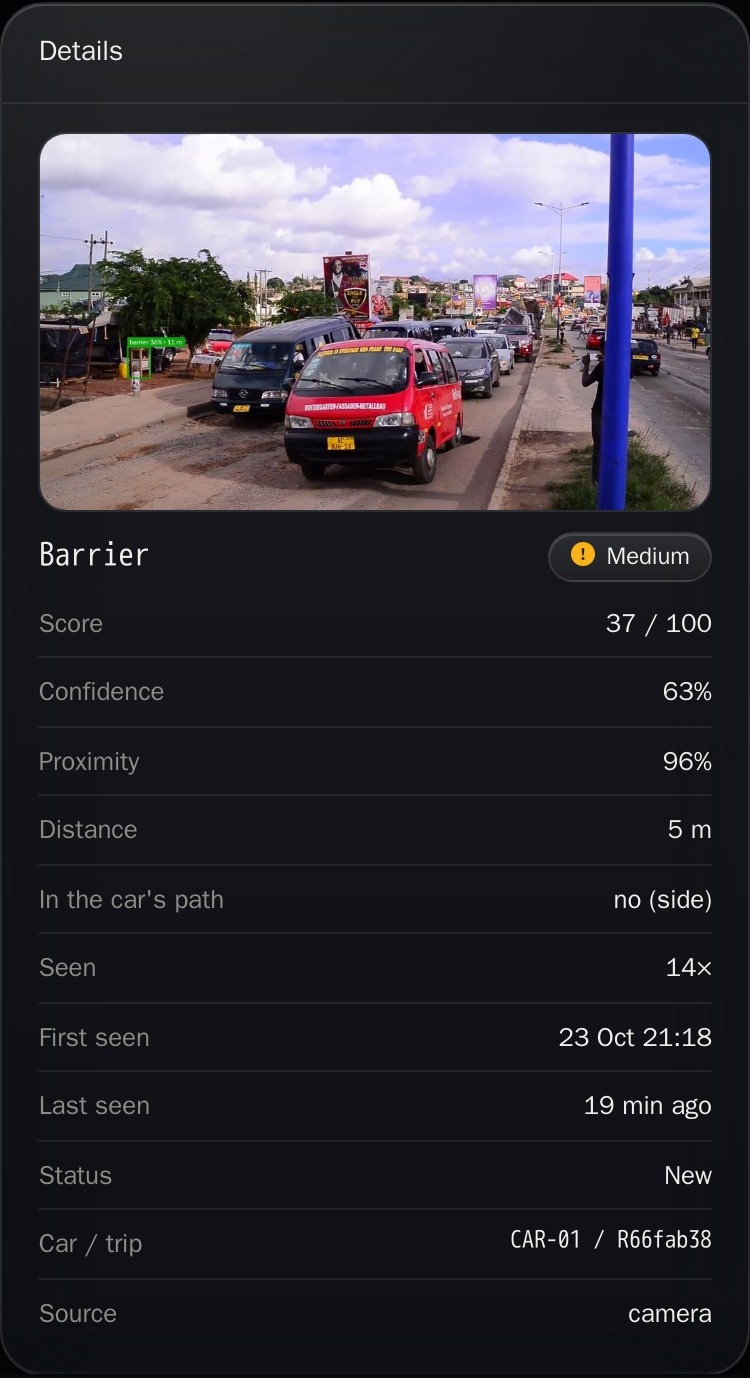
\includegraphics[width=\linewidth]{captures/obstacles_details_barrier.jpg}
  \caption{« Barrière » sur le côté : moyen}
\end{subfigure}\hfill
\begin{subfigure}[b]{0.32\linewidth}\centering
  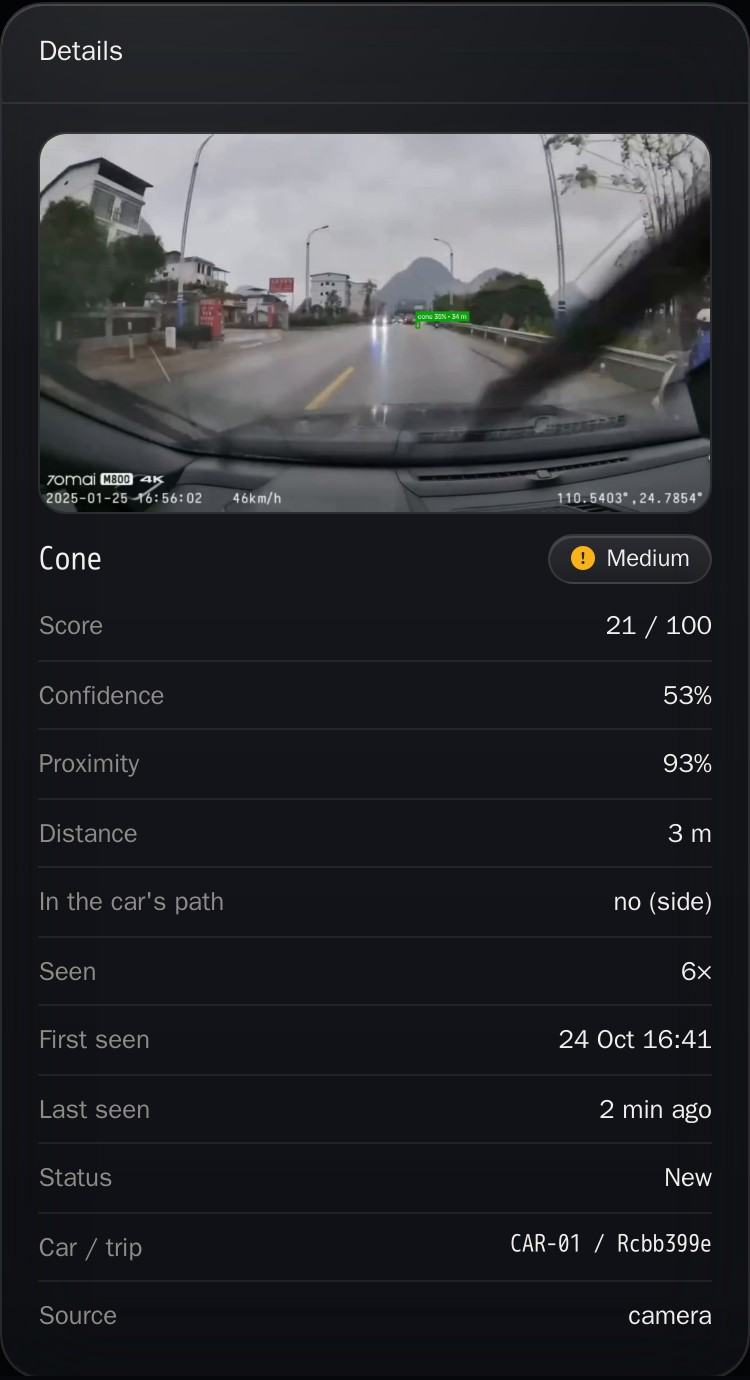
\includegraphics[width=\linewidth]{captures/obstacles_details_cone.jpg}
  \caption{Cône sur le côté : moyen}
\end{subfigure}

\vspace{0.2cm}
\begin{subfigure}[b]{\linewidth}\centering
  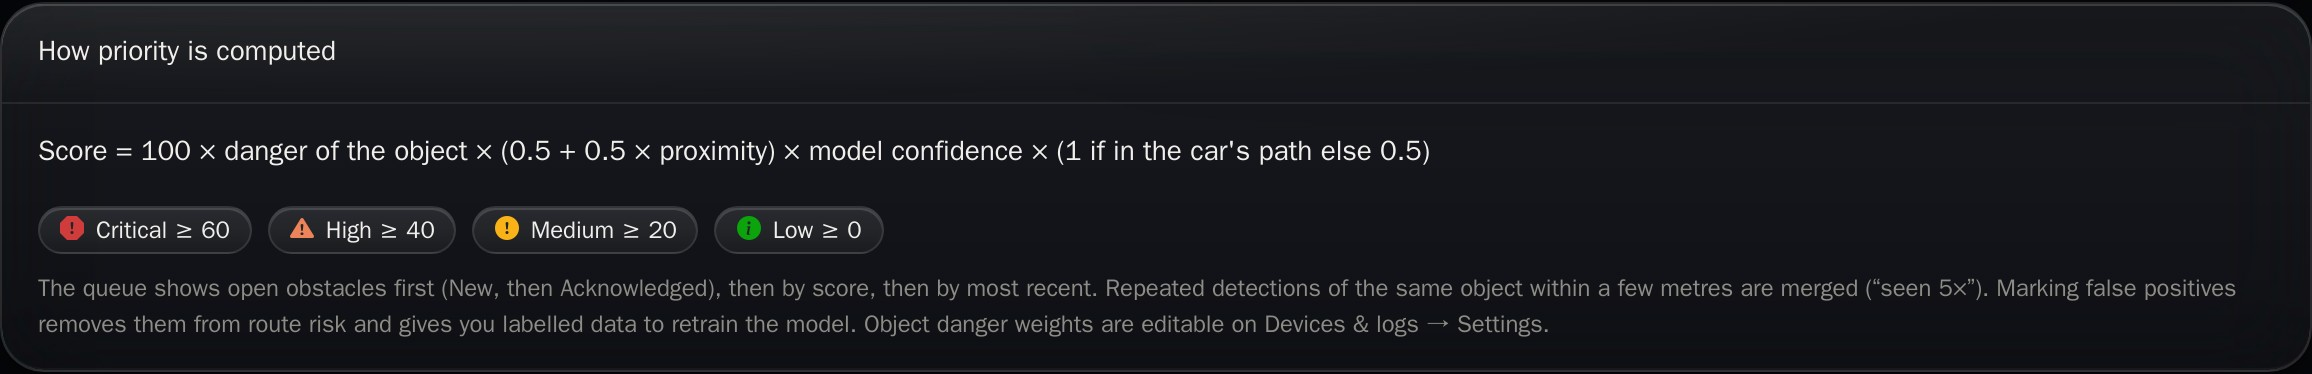
\includegraphics[width=\linewidth]{captures/obstacles_priority.jpg}
  \caption{Explication du calcul de la priorité}
\end{subfigure}
\caption{Niveaux de gravité et priorités : détail de trois obstacles détectés par la caméra embarquée}
\label{fig:obstacles-gravite}
\end{figure}

L'exemple de la « barrière » est instructif : l'instantané montre qu'il s'agit en réalité d'un poteau bleu. C'est
exactement le type d'erreur que l'opérateur peut signaler comme faux positif.

\subsection{Attribution des niveaux de priorité}
Le score détermine le niveau (critique, élevé, moyen, faible) et la file est triée par niveau puis par score. Les
indicateurs en tête de page comptent les obstacles ouverts de chaque niveau, le nombre d'obstacles revus et le taux de
faux positifs parmi eux (figure~\ref{fig:obstacles_kpis}). Les poids de danger étant réglables, l'opérateur peut
adapter la priorisation à son contexte ; tous les scores sont alors recalculés.

\capture{obstacles_kpis}{Indicateurs de la page Obstacles : obstacles ouverts par niveau, revues et faux positifs}

\subsection{Localisation et consultation des anomalies}
La sélection d'un obstacle affiche son détail : instantané annoté, classe et niveau, score, confiance, proximité,
distance, position par rapport à la trajectoire, nombre d'observations, dates, statut, véhicule, trajet et source.
La carte \emph{Where they are} situe tous les obstacles de la période. L'opérateur peut ensuite agir sur un ou
plusieurs obstacles sélectionnés : \textbf{Acknowledge} (pris en compte), \textbf{Resolve} (traité),
\textbf{False positive} (erreur du modèle) ou \textbf{Reopen}. Ces décisions modifient le risque utilisé par le
planificateur et alimentent l'évaluation des modèles.

\subsection{Filtrage et tri des obstacles}
La barre de filtres permet de choisir l'onglet (\emph{Needs review}, \emph{Acknowledged}, \emph{Closed},
\emph{All}), les niveaux affichés, les classes et la période (dernière heure, 24 heures, 7 jours, 30 jours, tout
l'historique) ; chaque colonne de la table peut être triée (figure~\ref{fig:obstacles_filters}).

\capture{obstacles_filters}{Barre de filtres de la page Obstacles}

% =================================================================================================
\section{Page Live Stats : statistiques et indicateurs}

La page \emph{Live stats} rassemble les indicateurs et graphiques statistiques (figure~\ref{fig:stats_real_ecran}).

\capture{stats_real_ecran}{Graphiques et indicateurs statistiques (monde réel)}

\subsection{Présentation des indicateurs statistiques}
En monde réel, les indicateurs sont : les véhicules en ligne, la distance parcourue et le nombre de trajets en
24 heures, la vitesse moyenne, le nombre moyen d'obstacles par heure, les manœuvres d'évitement et la batterie
moyenne. En prototype, ce sont l'état de la voiture, la source de données (caméra en direct ou démonstration), la
vitesse estimée, la cadence de la caméra, les parcours et les obstacles des dernières 24 heures
(figure~\ref{fig:stats-kpi}).

\begin{figure}[H]
\centering
\begin{subfigure}[b]{\linewidth}\centering
  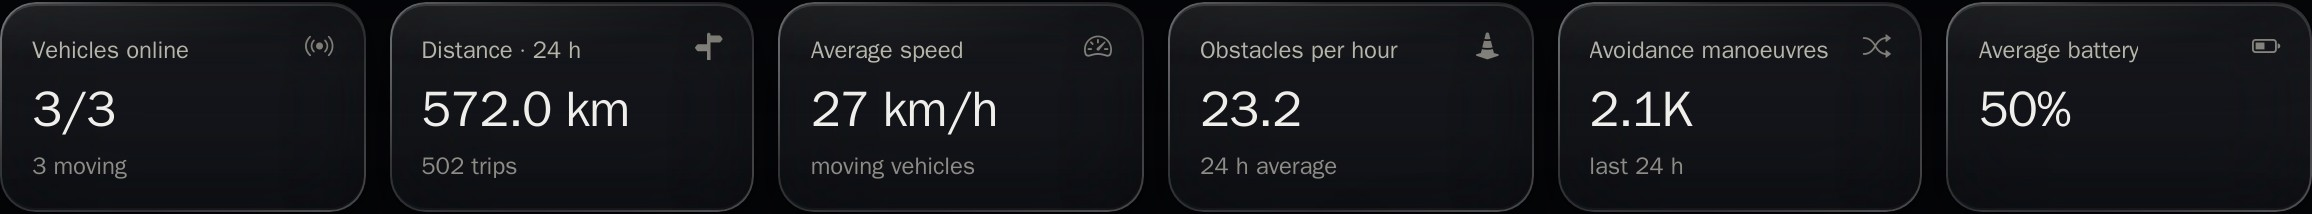
\includegraphics[width=\linewidth]{captures/stats_kpi_real.jpg}
  \caption{Monde réel}
\end{subfigure}

\vspace{0.2cm}
\begin{subfigure}[b]{\linewidth}\centering
  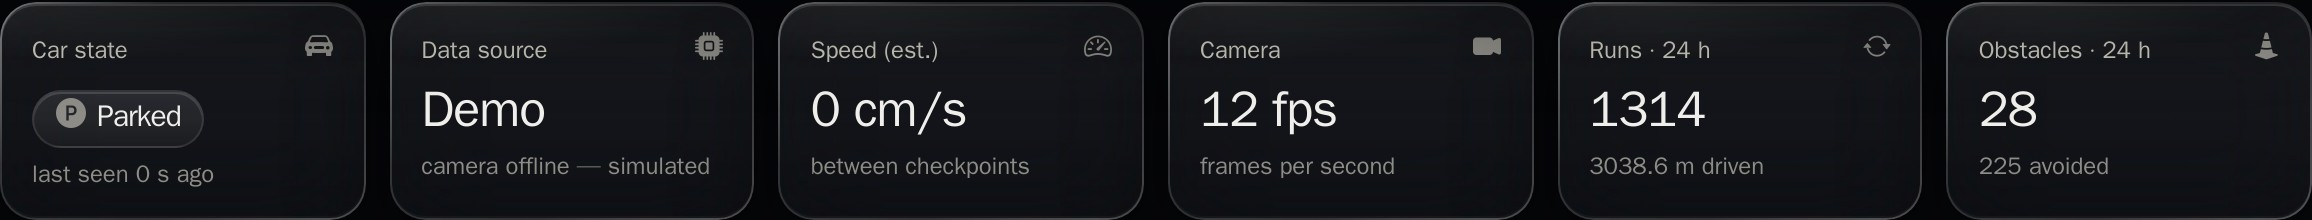
\includegraphics[width=\linewidth]{captures/stats_kpi_proto.jpg}
  \caption{Prototype}
\end{subfigure}
\caption{Indicateurs statistiques dans les deux environnements}
\label{fig:stats-kpi}
\end{figure}

\subsection{Nombre et répartition des obstacles détectés}
Le graphique \emph{Obstacles per hour} montre le nombre d'obstacles détectés par heure sur les dernières 24 heures,
ce qui fait apparaître les périodes chargées ; le graphique \emph{Obstacles by object} donne leur répartition par
classe sur 7 jours (figure~\ref{fig:stats-obstacles}).

\begin{figure}[H]
\centering
\begin{subfigure}[b]{0.49\linewidth}\centering
  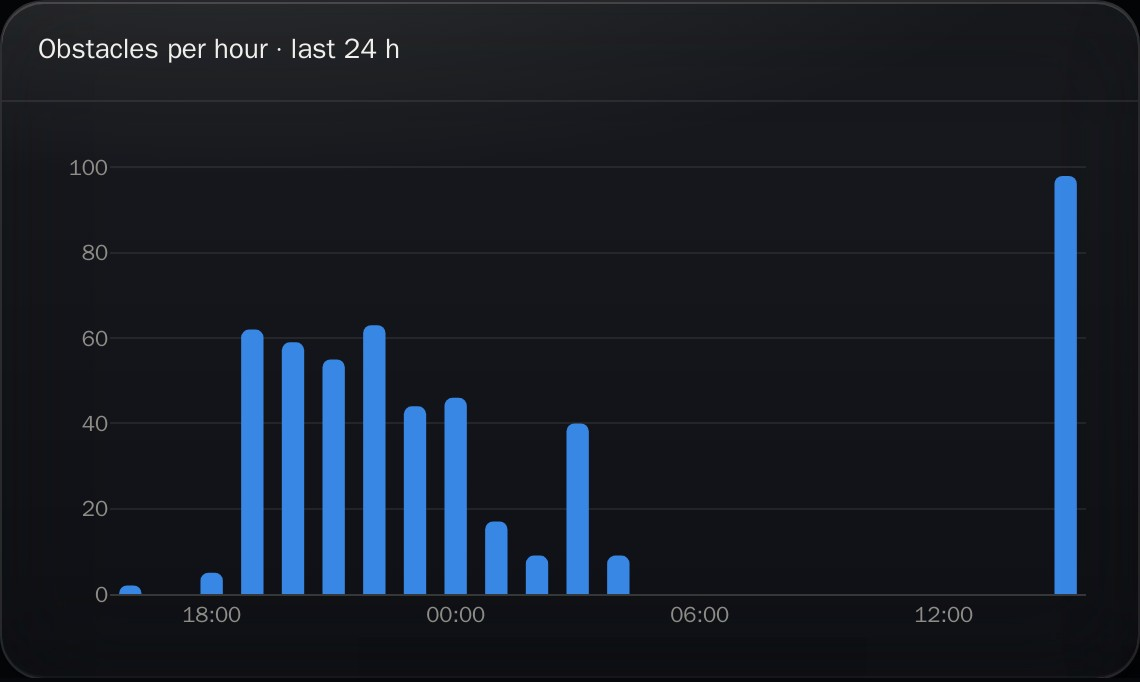
\includegraphics[width=\linewidth]{captures/stats_hourly.jpg}
  \caption{Obstacles par heure (24 h)}
\end{subfigure}\hfill
\begin{subfigure}[b]{0.49\linewidth}\centering
  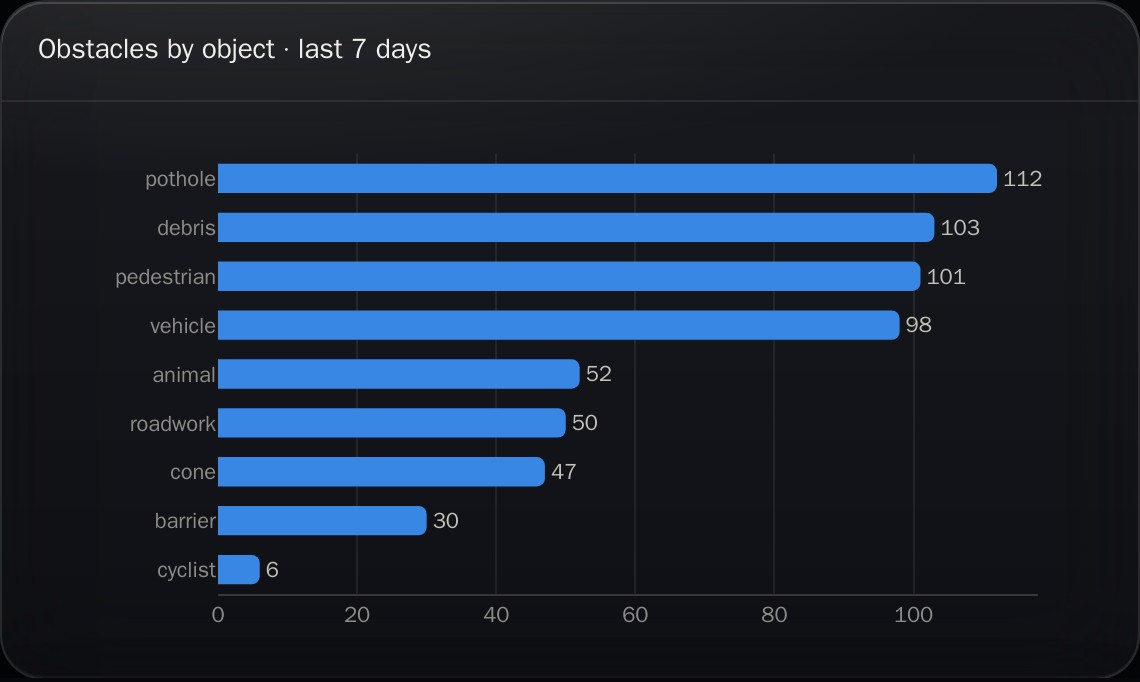
\includegraphics[width=\linewidth]{captures/stats_classes.jpg}
  \caption{Obstacles par classe (7 jours)}
\end{subfigure}
\caption{Nombre et répartition des obstacles détectés}
\label{fig:stats-obstacles}
\end{figure}

\subsection{Distribution des anomalies par gravité et priorité}
Le graphique \emph{Severity mix} montre, pour chaque jour, la part de chaque niveau de gravité parmi les obstacles
détectés (figure~\ref{fig:stats-severite}). Il permet de suivre l'évolution de la dangerosité et non seulement du
volume.

\subsection{Analyse des données de suivi des véhicules}
La chronologie \emph{Vehicle state} montre l'état de chaque véhicule (en route, en évitement, arrêté, en charge) sur
les 15 dernières minutes, le graphique \emph{Speed} leur vitesse sur 5 minutes, et le graphique des trajets par jour
l'activité de la flotte (figure~\ref{fig:stats-severite}).

\begin{figure}[H]
\centering
\begin{subfigure}[b]{0.49\linewidth}\centering
  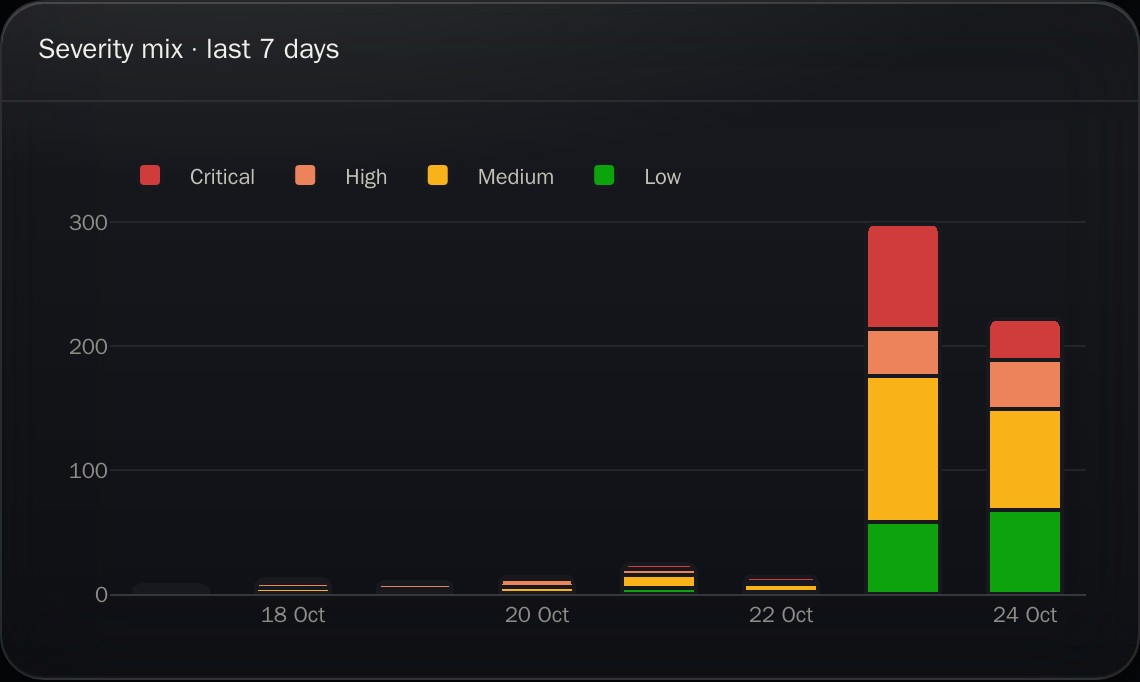
\includegraphics[width=\linewidth]{captures/stats_severity.jpg}
  \caption{Répartition par gravité}
\end{subfigure}\hfill
\begin{subfigure}[b]{0.49\linewidth}\centering
  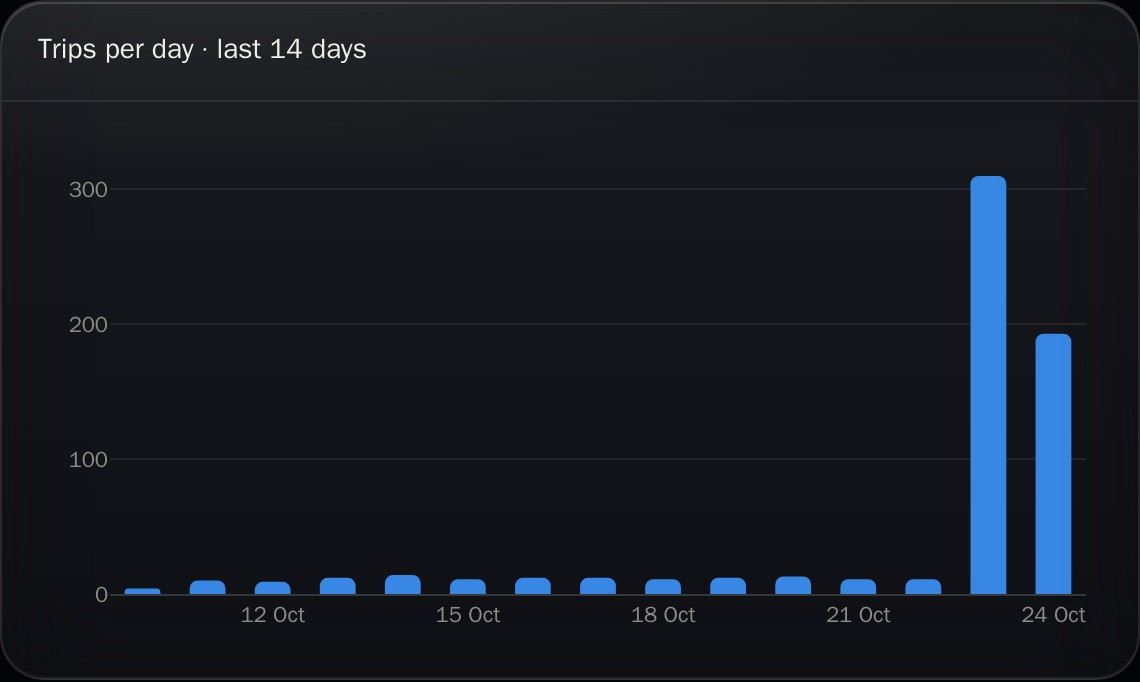
\includegraphics[width=\linewidth]{captures/stats_trips.jpg}
  \caption{Trajets par jour}
\end{subfigure}

\vspace{0.2cm}
\begin{subfigure}[b]{0.49\linewidth}\centering
  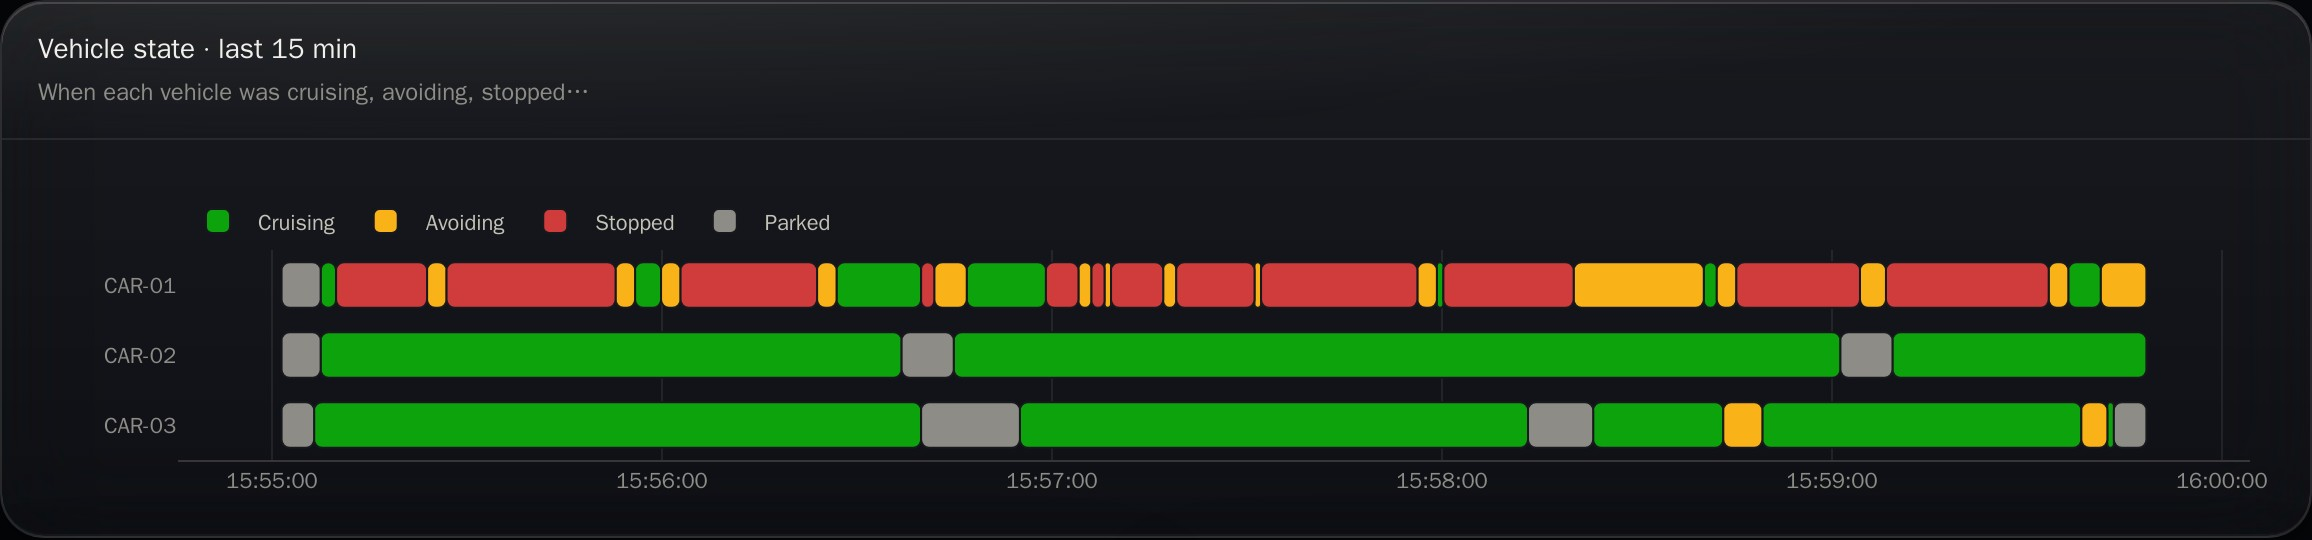
\includegraphics[width=\linewidth]{captures/stats_states.jpg}
  \caption{États des véhicules (15 min)}
\end{subfigure}\hfill
\begin{subfigure}[b]{0.49\linewidth}\centering
  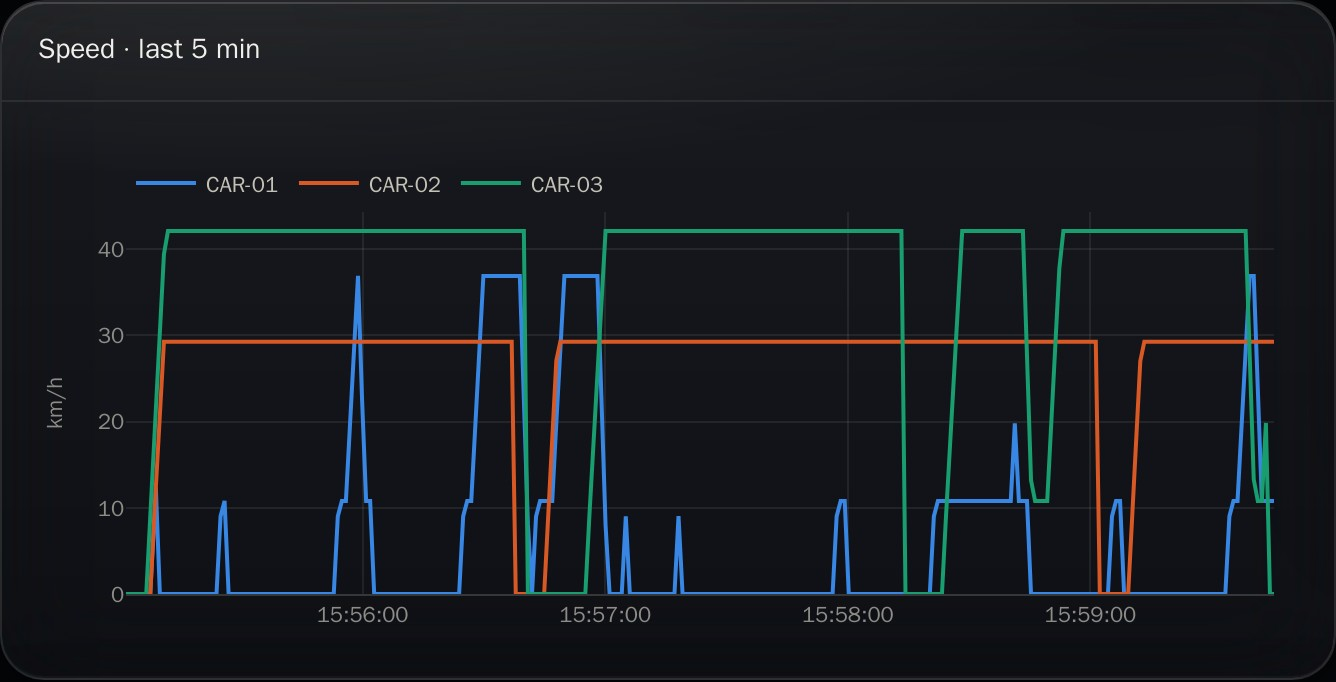
\includegraphics[width=\linewidth]{captures/stats_speed.jpg}
  \caption{Vitesse des véhicules (5 min)}
\end{subfigure}
\caption{Gravité des anomalies et données de suivi des véhicules}
\label{fig:stats-severite}
\end{figure}

\subsection{Visualisation graphique des statistiques}
Les graphiques sont construits avec Plotly et partagent une même charte : fond transparent sur les panneaux,
quadrillage discret, palette de couleurs catégorielles distinctes pour les séries, couleurs de gravité réservées aux
niveaux (rouge, orange, jaune, vert) et infobulles au survol. Les valeurs sont toujours accompagnées de leur unité.

\subsection{Comparaison des résultats entre les deux environnements}
Le changement d'environnement s'applique aussi aux statistiques : la même page présente les données de la flotte
simulée ou celles de la voiture du prototype (figure~\ref{fig:stats-env}). La comparaison doit tenir compte de la
nature des données : les statistiques du monde réel décrivent une flotte simulée dont seul CAR-01 voit de vraies
images, alors que celles du prototype décrivent des parcours réels sur la piste lorsque la caméra est connectée.

\begin{figure}[H]
\centering
\begin{subfigure}[b]{0.49\linewidth}\centering
  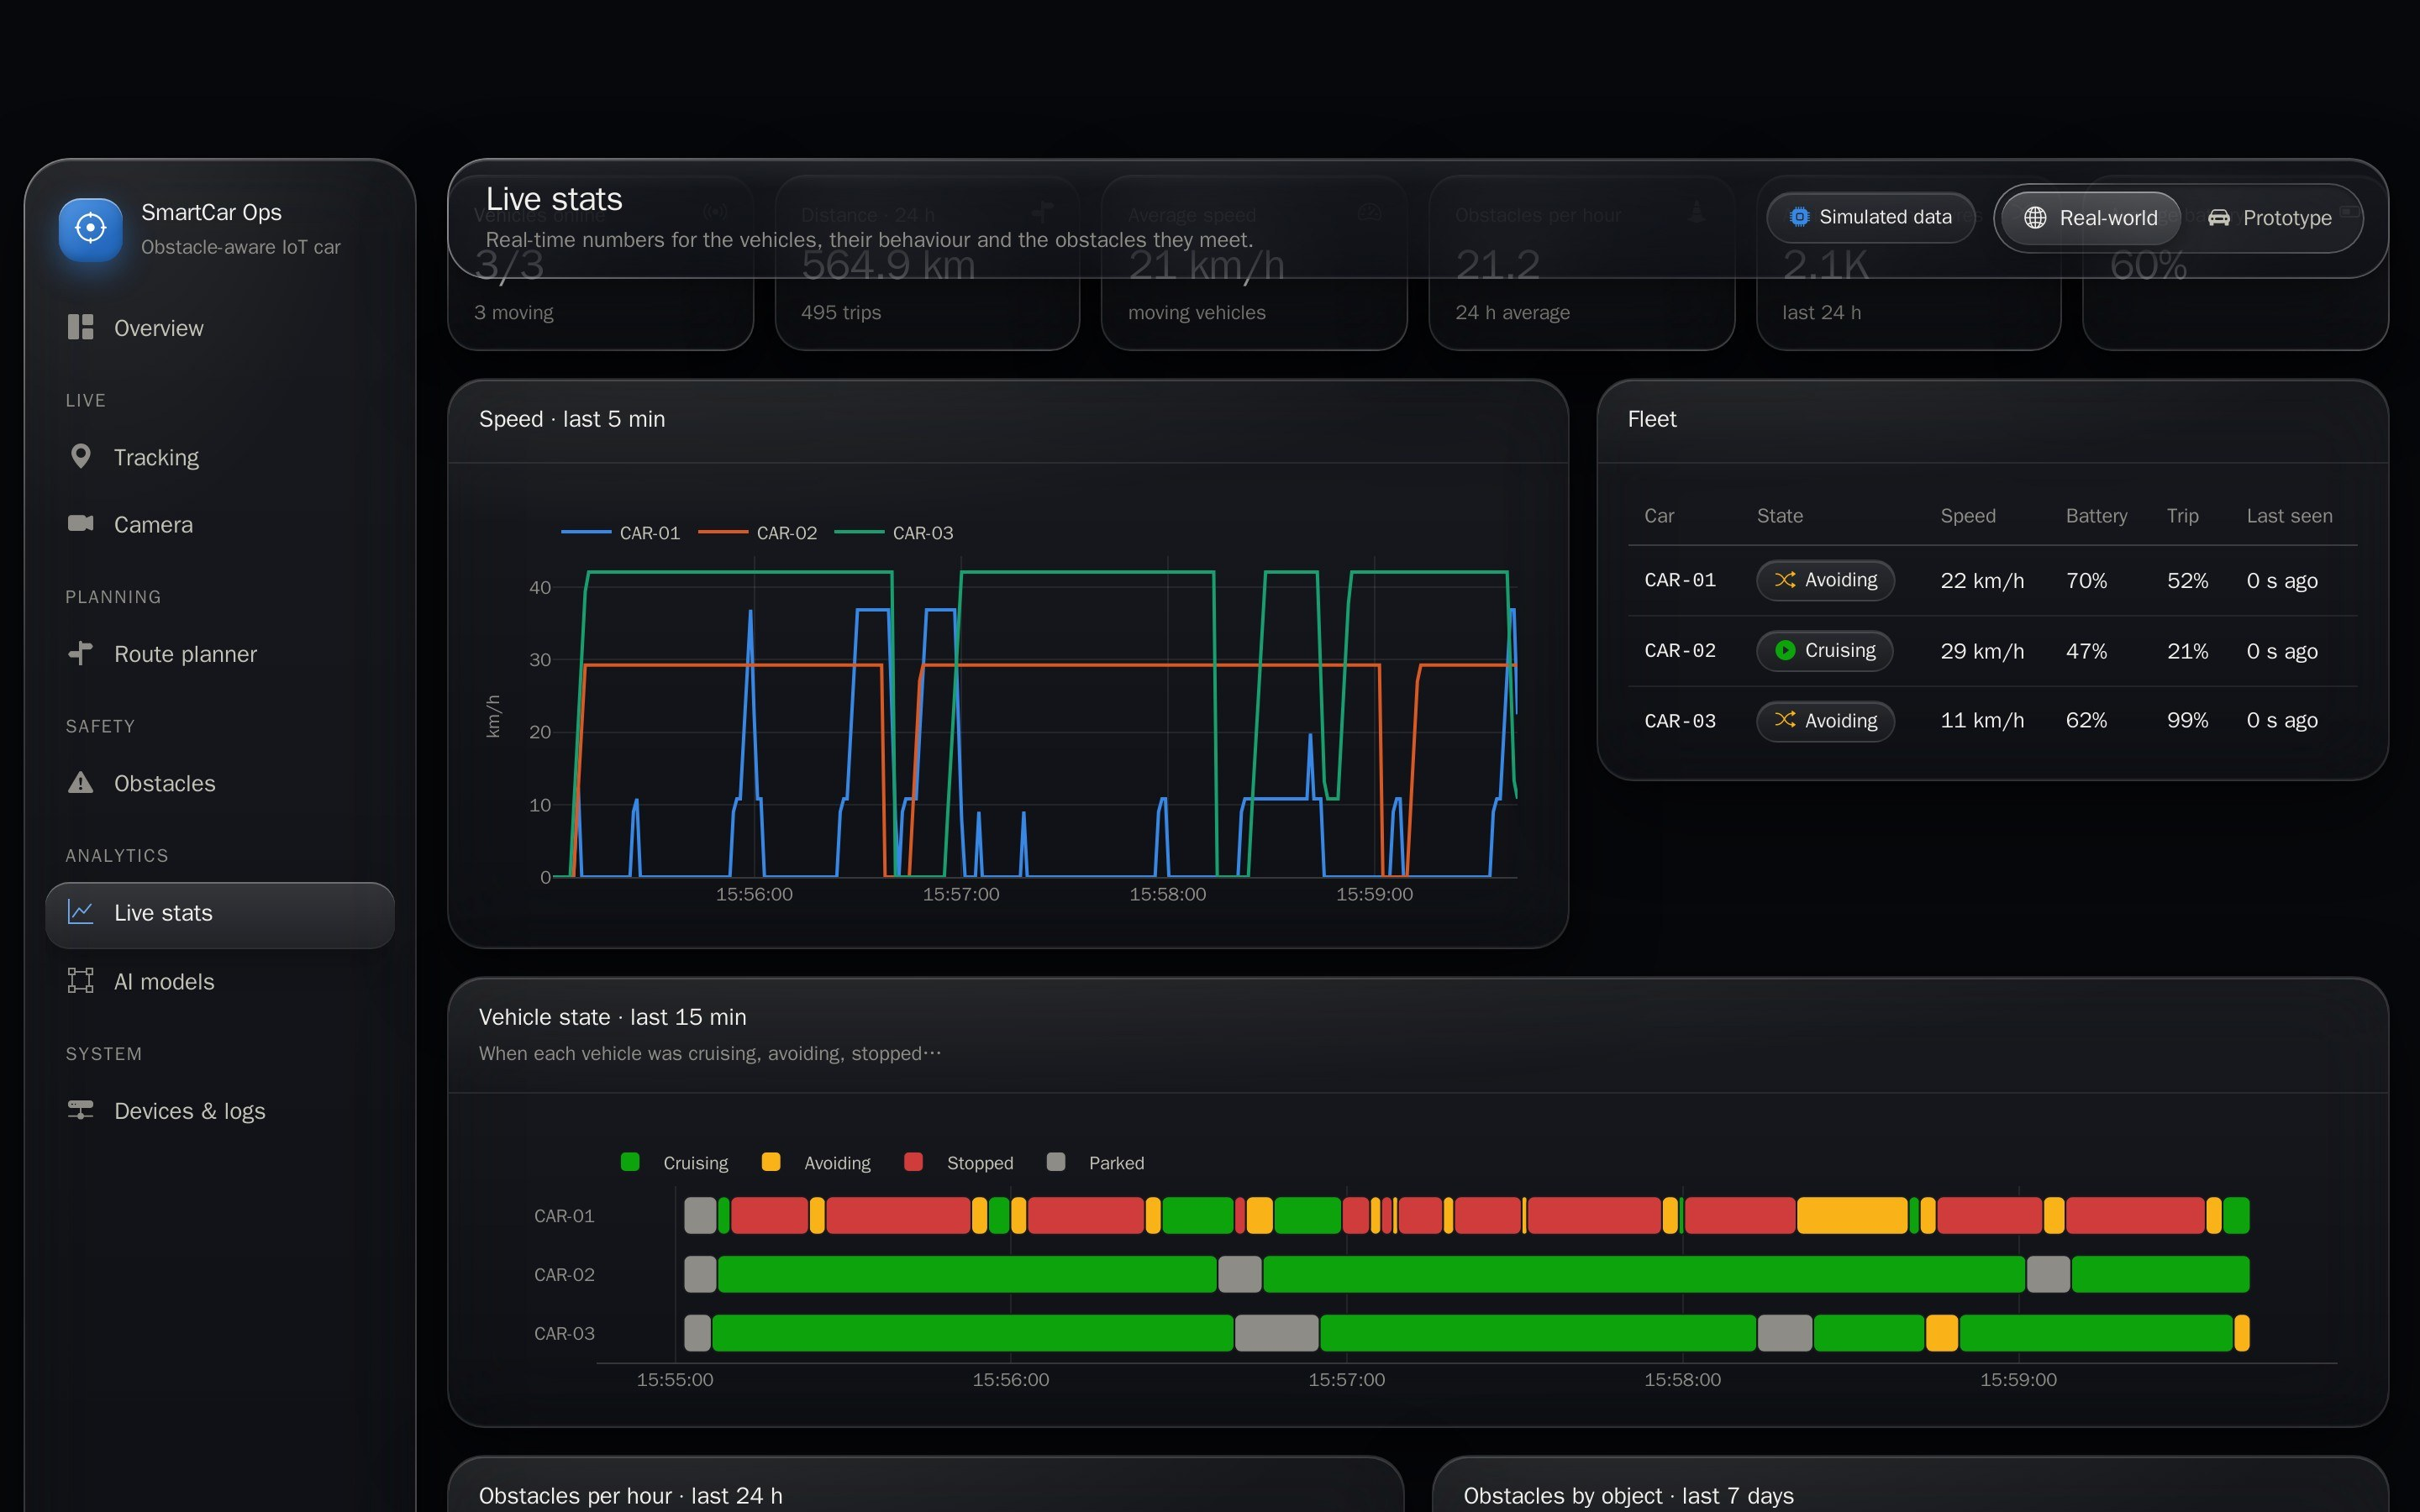
\includegraphics[width=\linewidth]{captures/stats_real_ecran.jpg}
  \caption{Monde réel}
\end{subfigure}\hfill
\begin{subfigure}[b]{0.49\linewidth}\centering
  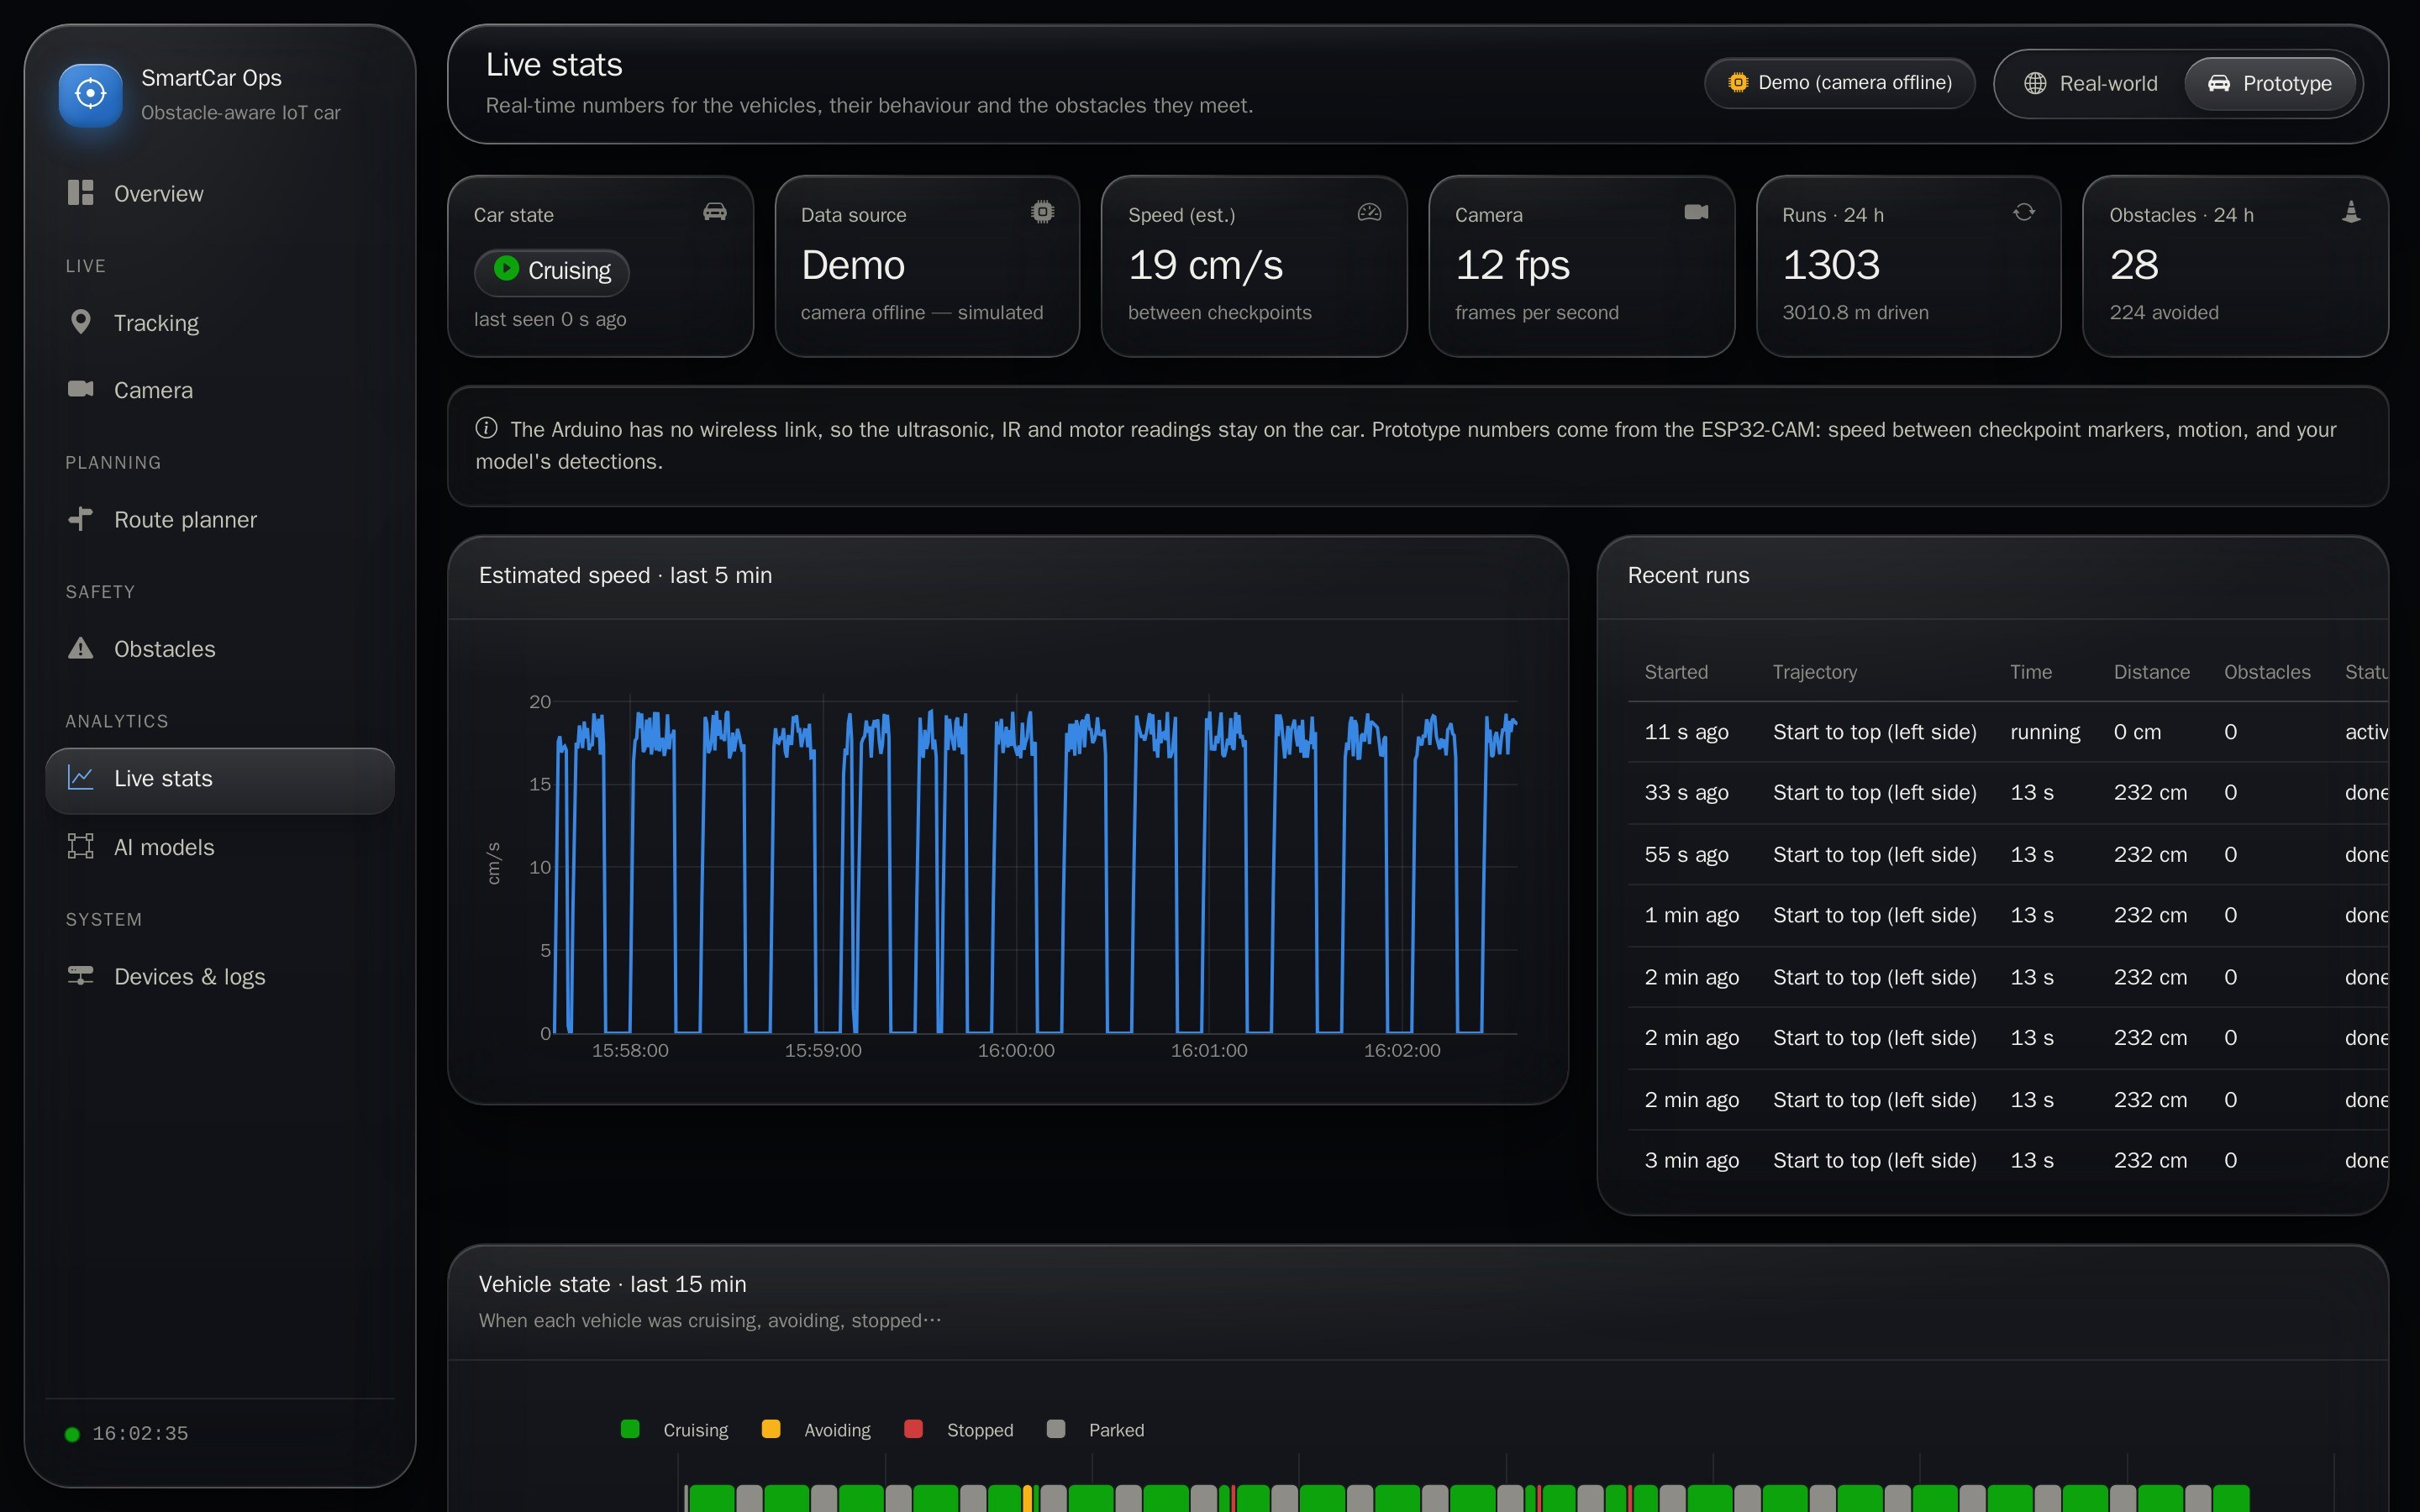
\includegraphics[width=\linewidth]{captures/stats_proto_ecran.jpg}
  \caption{Prototype}
\end{subfigure}
\caption{Page Live stats dans les deux environnements}
\label{fig:stats-env}
\end{figure}

% =================================================================================================
\section{Page AI Models : gestion des modèles d'intelligence artificielle}

La page \emph{AI models} présente, pour l'environnement choisi, chaque modèle avec son évaluation hors ligne, puis son
comportement sur la route (figure~\ref{fig:models_hazards}).

\capture{models_hazards}{Page de présentation des modèles : détecteur d'anomalies routières}

\subsection{Présentation des modèles utilisés}
Chaque modèle est présenté par une carte : nom, architecture, version, date d'entraînement, taille d'entrée, nombre
d'images, répartition entraînement / validation / test, durée d'entraînement et matériel, sources des données et
badge indiquant l'origine des métriques (évaluation sur un ensemble de test, modèle préentraîné, entraînement en
attente). Ces informations proviennent du registre \texttt{models/registry.json}, mis à jour par les notebooks
d'entraînement.

\subsection{Modèles YOLO26 pour les données réelles}
En monde réel, deux cartes sont affichées : le détecteur des usagers de la route (YOLO26n préentraîné sur COCO, avec
la liste des classes utilisées) et le détecteur d'anomalies routières (YOLO26s affiné). Pour ce dernier, deux
rangées de métriques sont présentées et clairement libellées : le meilleur réglage hors ligne (960 px avec TTA) et le
réglage temps réel utilisé dans l'application (640 px) (figure~\ref{fig:models_users}).

\capture[0.9]{models_users}{Carte du modèle des usagers de la route (préentraîné sur COCO)}

\subsection{Modèle YOLO26n pour le prototype}
En mode prototype, la carte du modèle des obstacles de la piste présente ses métriques sur les images de test
d'origine et sur leurs versions au style ESP32-CAM, la précision moyenne par classe et la matrice de confusion
(figure~\ref{fig:models_toy}).

\capture{models_toy}{Carte du modèle du prototype}

\subsection{Configuration et chargement des modèles}
La configuration est entièrement déclarative : chaque environnement dispose d'un profil qui liste ses modèles ONNX,
leur taille d'entrée, leur seuil de confiance et la correspondance de leurs classes. Un nouveau modèle se déploie en
copiant son fichier ONNX et en mettant à jour le profil, puis en redémarrant l'application ; un modèle manquant est
signalé sans bloquer le reste.

\subsection{Affichage des informations et des performances}
Les métriques hors ligne (précision, rappel, mAP@50, mAP@50-95, temps d'inférence sur GPU) sont complétées par deux
graphiques : la précision moyenne par classe et la matrice de confusion, normalisée par classe réelle et calculée au
seuil de confiance utilisé dans l'application. Le panneau \emph{On the road · last 7 days} mesure le comportement
réel : nombre de détections, confiance moyenne, nombre d'obstacles revus par l'opérateur, taux de faux positifs par
classe et modèle en cours d'utilisation (figure~\ref{fig:models_live}).

\capture{models_live}{Comportement des modèles sur la route (7 derniers jours)}

\subsection{Comparaison des résultats des modèles}
La page permet de confronter deux points de vue complémentaires : l'évaluation hors ligne, mesurée une fois sur un
ensemble de test annoté, et l'évaluation en service, construite progressivement à partir des revues de l'opérateur.
Un écart entre les deux (par exemple un taux de faux positifs élevé pour une classe) signale les classes à enrichir
lors du prochain entraînement ; les obstacles marqués comme faux positifs constituent alors des exemples
directement réutilisables.

% =================================================================================================
\section{Page Devices \& Logs : périphériques et journaux du système}

La page \emph{Devices \& logs} comporte trois onglets : \emph{Devices}, \emph{Event log} et \emph{Settings}
(figure~\ref{fig:system_devices_grid}).

\capture{system_devices_grid}{Périphériques et services du système}

\subsection{Présentation des périphériques connectés}
L'onglet \emph{Devices} présente une carte par équipement ou service : la caméra embarquée de CAR-01 (source, clip,
cadence vidéo et cadence d'analyse), l'ESP32-CAM (adresse IP, méthode de découverte, cadence, résolution, dernière
image), l'Arduino UNO (rappel de son rôle et de ses broches, sans liaison directe avec le serveur), les données du
prototype (piste, trajectoire active, points de passage), le simulateur du monde réel (véhicules, réseau routier), les
modèles chargés et la base de données (nombre de trajets, de points, d'obstacles et d'événements).

\subsection{Suivi de l'état des composants et des dispositifs}
Chaque carte porte un badge d'état (en ligne, hors ligne, en lecture, démonstration…) mis à jour en continu. Les
problèmes sont ainsi visibles immédiatement : une caméra introuvable, un modèle non chargé ou une source vidéo vide.

\subsection{Consultation des journaux d'exécution}
L'onglet \emph{Event log} affiche le journal des événements de l'environnement choisi : date, niveau (information,
avertissement, critique), catégorie et message. Il peut être filtré par niveau et par catégorie
(figure~\ref{fig:system_events_panel}).

\capture{system_events_panel}{Journal des événements}

\subsection{Gestion des événements et des erreurs}
Les événements sont enregistrés par tous les composants : début et fin de trajet, passage aux points de passage,
obstacle de niveau élevé ou critique, connexion et perte de la caméra, changement de statut d'obstacles, erreurs du
détecteur. Les erreurs ne bloquent pas l'application : une caméra perdue est recherchée à nouveau automatiquement, et
une erreur de modèle est signalée une seule fois dans le journal puis affichée sur la page Camera.

\subsection{Diagnostic et surveillance du système}
L'onglet \emph{Settings} permet de régler les poids de danger des classes, puis de recalculer tous les scores, et de
régénérer les données de démonstration (figure~\ref{fig:system_weights}). Associés à la page \emph{Camera} (état de la
connexion) et à la page \emph{AI models} (modèles chargés), ces outils permettent de diagnostiquer rapidement l'état du
système.

\capture[0.55]{system_weights}{Réglage des poids de danger des classes}

% =================================================================================================
\section{Synthèse des fonctionnalités de l'application}

\subsection{Interconnexion des différentes pages}
Les pages ne sont pas indépendantes : elles partagent les mêmes données et les actions faites sur l'une se
répercutent sur les autres (figure~\ref{fig:interactions}). Les détections de la page \emph{Camera} deviennent des
obstacles ; les décisions prises dans la page \emph{Obstacles} modifient le risque utilisé par le \emph{Route
planner} et alimentent le taux de faux positifs de la page \emph{AI models} ; les poids réglés dans \emph{Devices \&
logs} changent la priorité de tous les obstacles ; la trajectoire active choisie dans le planificateur sert à la
localisation de la voiture du prototype.

\begin{figure}[H]
\centering
\resizebox{0.95\linewidth}{!}{% Interactions entre les modules de l'application (chapitre 4)
\begin{tikzpicture}[
  p/.style={bloc,font=\footnotesize,minimum width=2.9cm,text width=2.7cm,minimum height=1.05cm,fill=bleufst!8},
  lb/.style={font=\scriptsize\itshape,text=encre!80,fill=white,inner sep=1pt,align=center}]
  \node[bloc,minimum width=3.8cm,text width=3.6cm,fill=gris!12,draw=gris,font=\footnotesize,minimum height=1.6cm] (core)
       at (0,0) {\textbf{Données partagées}\\hub en mémoire\\SQLite, réglages};
  \node[p] (ov)  at (0,4.0)    {Overview};
  \node[p] (tr)  at (-5.0,2.6) {Tracking};
  \node[p] (cam) at (-5.6,-0.6) {Camera};
  \node[p] (ob)  at (-3.4,-3.8) {Obstacles};
  \node[p] (pl)  at (3.4,-3.8) {Route planner};
  \node[p] (st)  at (5.0,2.6)  {Live stats};
  \node[p] (md)  at (5.6,-0.6)   {AI models};
  \node[p] (sys) at (0,-5.6)    {Devices \& logs};
  \foreach \n in {ov,tr,cam,ob,pl,st,md,sys} \draw[thick,draw=gris!70,dashed] (\n) -- (core);
  \draw[fleche] (cam) -- node[lb,left] {détections\\$\rightarrow$ obstacles} (ob);
  \draw[fleche] (ob) -- node[lb,below] {statut, gravité\\$\rightarrow$ risque des segments} (pl);
  \draw[fleche] ([yshift=0.25cm]ob.east) -- node[lb,pos=0.62,above,sloped] {revues $\rightarrow$ faux positifs} (md.south west);
  \draw[fleche] (sys) -- node[lb,left] {poids de danger\\$\rightarrow$ scores recalculés} (ob.south);
  \draw[fleche] ([yshift=0.3cm]pl.west) -- node[lb,pos=0.5,above,sloped] {trajectoire active (prototype)} (cam.south east);
  \draw[fleche] (tr) -- node[lb,above,sloped] {trajets} (ov);
  \draw[fleche] (ob.north) to[out=95,in=-120] node[lb,pos=0.85,left] {à traiter} (ov.south west);
  \draw[fleche] (cam.north) -- node[lb,left] {état du véhicule} (tr.south);
\end{tikzpicture}
}
\caption{Interactions entre les modules de l'application}
\label{fig:interactions}
\end{figure}

\subsection{Circulation des données entre les composants}
Les données suivent toujours le même chemin : acquisition par les services d'arrière-plan, analyse par les modèles,
enregistrement dans le hub et la base de données, lecture par les pages à chaque rafraîchissement, puis retour des
décisions de l'opérateur vers la base. Cette séparation entre acquisition et affichage garantit que l'interface reste
fluide quelle que soit la vitesse des modèles, et que plusieurs opérateurs peuvent consulter l'application en même
temps.

\subsection{Apports de l'application au système intelligent}
\app{} transforme les sorties brutes des modèles (des boîtes et des scores) en informations exploitables : des
obstacles localisés, dédupliqués, hiérarchisés et suivis dans le temps, intégrés à la planification des itinéraires.
Elle ferme la boucle entre la perception et la décision, et entre l'opérateur et les modèles, puisque ses revues
préparent les prochains entraînements. Enfin, en gérant les deux environnements avec la même chaîne logicielle, elle
montre que la solution validée sur le prototype est transposable à des données routières réelles.

\chapconclusion
Ce chapitre a présenté l'application \app : ses choix technologiques (Dash, Plotly, Docker), son architecture en
couches, la gestion de ses données et ses huit pages. L'application exécute les modèles en temps réel, priorise les
obstacles selon un score explicable, en tient compte dans la planification des itinéraires et permet à l'opérateur de
superviser aussi bien une flotte sur des routes réelles que la voiture du prototype.
